\documentclass[12pt,a4paper]{article}

% ── Encodage et langue ──
\usepackage[utf8]{inputenc}
\usepackage[T1]{fontenc}
\usepackage[french]{babel}

% ── Mise en page ──
\usepackage[margin=2.5cm]{geometry}
\usepackage{setspace}
\onehalfspacing
\usepackage{parskip}

% ── Maths ──
\usepackage{amsmath,amssymb,amsthm,mathtools}
\usepackage{bm}

% ── Figures et tableaux ──
\usepackage{graphicx}
\graphicspath{{../results/figures/}}
\usepackage{float}
\usepackage{booktabs}
\usepackage{array}
\usepackage{multirow}
\usepackage{caption}
\usepackage{subcaption}

% ── Couleurs et liens ──
\usepackage[dvipsnames,svgnames,x11names]{xcolor}
\usepackage[colorlinks=true,linkcolor=Navy,citecolor=Navy,urlcolor=Navy]{hyperref}

% ── Couleurs du projet ──
\definecolor{eccblue}{RGB}{0,51,102}
\definecolor{eccgold}{RGB}{198,146,20}
\definecolor{ecclight}{RGB}{230,240,250}
\definecolor{eccdark}{RGB}{20,30,50}
\definecolor{sectioncolor}{RGB}{0,70,130}
\definecolor{boxbg}{RGB}{240,245,252}
\definecolor{boxborder}{RGB}{0,80,150}

% ── Boites decoratives ──
\usepackage[most]{tcolorbox}
\tcbset{
  defstyle/.style={
    colback=ecclight,
    colframe=eccblue,
    fonttitle=\bfseries,
    arc=2mm,
    boxrule=0.8pt,
    left=8pt, right=8pt, top=6pt, bottom=6pt,
  },
  propstyle/.style={
    colback=eccgold!8,
    colframe=eccgold!70!black,
    fonttitle=\bfseries,
    arc=2mm,
    boxrule=0.8pt,
    left=8pt, right=8pt, top=6pt, bottom=6pt,
  },
  rmqstyle/.style={
    colback=gray!5,
    colframe=gray!50,
    fonttitle=\bfseries\itshape,
    arc=1mm,
    boxrule=0.5pt,
    left=8pt, right=8pt, top=4pt, bottom=4pt,
  },
  eqbox/.style={
    colback=eccblue!4,
    colframe=eccblue!50,
    arc=2mm,
    boxrule=0.6pt,
    left=6pt, right=6pt, top=8pt, bottom=8pt,
  },
}

% ── Titres colores ──
\usepackage{titlesec}
\titleformat{\section}
  {\LARGE\bfseries\color{eccblue}}
  {\thesection.}{0.5em}{}
  [\vspace{-0.5em}{\color{eccgold}\rule{\linewidth}{1.5pt}}]
\titleformat{\subsection}
  {\Large\bfseries\color{sectioncolor}}
  {\thesubsection}{0.5em}{}
\titleformat{\subsubsection}
  {\large\bfseries\color{eccblue!80}}
  {\thesubsubsection}{0.5em}{}

% ── Code ──
\usepackage{listings}
\lstset{
  basicstyle=\ttfamily\small,
  frame=single,
  breaklines=true,
  language=Python,
  backgroundcolor=\color{gray!5},
}

% ── Biblio ──
\usepackage[numbers,sort&compress]{natbib}

% ── En-tete / pied de page ──
\usepackage{fancyhdr}
\pagestyle{fancy}
\fancyhf{}
\fancyhead[L]{\small\color{eccblue}\textit{Sujet 3 --- Mod\`eles de diffusion}}
\fancyhead[R]{\small\color{eccblue}\textit{ML --- ECC 2026-2027}}
\fancyfoot[C]{\color{eccblue}\thepage}
\renewcommand{\headrulewidth}{0.4pt}
\renewcommand{\headrule}{\hbox to\headwidth{\color{eccgold}\leaders\hrule height \headrulewidth\hfill}}

% ── Theoremes avec tcolorbox ──
\newcounter{defctr}[section]
\renewcommand{\thedefctr}{\thesection.\arabic{defctr}}
\newcounter{propctr}[section]
\renewcommand{\thepropctr}{\thesection.\arabic{propctr}}
\newcounter{rmqctr}[section]
\renewcommand{\thermqctr}{\thesection.\arabic{rmqctr}}

\newenvironment{definition}[1][]
  {\refstepcounter{defctr}\begin{tcolorbox}[defstyle,title={D\'efinition~\thedefctr\if\relax\detokenize{#1}\relax\else~--- #1\fi}]}
  {\end{tcolorbox}}

\newenvironment{proposition}[1][]
  {\refstepcounter{propctr}\begin{tcolorbox}[propstyle,title={Proposition~\thepropctr\if\relax\detokenize{#1}\relax\else~--- #1\fi}]}
  {\end{tcolorbox}}

\newenvironment{remarque}[1][]
  {\refstepcounter{rmqctr}\begin{tcolorbox}[rmqstyle,title={Remarque~\thermqctr\if\relax\detokenize{#1}\relax\else~--- #1\fi}]}
  {\end{tcolorbox}}

% ── Commandes utiles ──
\newcommand{\E}{\mathbb{E}}
\newcommand{\R}{\mathbb{R}}
\newcommand{\N}{\mathcal{N}}
\newcommand{\bx}{\bm{x}}
\newcommand{\bz}{\bm{z}}
\newcommand{\beps}{\bm{\epsilon}}
\DeclareMathOperator*{\argmin}{arg\,min}

\begin{document}

% ══════════════════════════════════════════════════════════
% PAGE DE TITRE
% ══════════════════════════════════════════════════════════
\thispagestyle{empty}
\begin{center}

% ── Bande superieure ──
\noindent\colorbox{eccblue}{%
  \parbox{\dimexpr\linewidth-2\fboxsep}{%
    \centering\vspace{12pt}
    {\color{white}\Large\textsc{\'Ecole Centrale Casablanca}}\\[6pt]
    {\color{eccgold}\large Ann\'ee universitaire 2026--2027 --- Semestre 9}\\[4pt]
    {\color{white}\normalsize Fili\`ere : Industrie 4.0}
    \vspace{10pt}
  }%
}

\vspace{2cm}

% ── Titre principal ──
{\color{eccgold}\rule{\linewidth}{2pt}}\\[0.5cm]
{\color{eccblue}\LARGE \textbf{Mod\`eles de diffusion pour la pr\'evision\\[4pt] probabiliste et l'imputation de\\[4pt] s\'eries temporelles}}\\[0.4cm]
{\color{eccdark}\Large \textbf{Application aux donn\'ees financi\`eres}}\\[0.3cm]
{\color{eccgold}\rule{\linewidth}{2pt}}

\vspace{0.8cm}

% ── Badge sujet ──
\begin{tcolorbox}[
  colback=eccgold!10,
  colframe=eccgold,
  width=8cm,
  arc=3mm,
  boxrule=1pt,
  halign=center,
]
{\large\bfseries\color{eccblue} Sujet 3 --- Projet de Machine Learning}
\end{tcolorbox}

\vspace{1.2cm}

% ── Etudiants ──
\begin{tcolorbox}[
  colback=ecclight,
  colframe=eccblue,
  width=12cm,
  arc=2mm,
  boxrule=0.8pt,
  title={\centering Groupe 24 --- \'Equipe projet},
  fonttitle=\bfseries\color{white},
  coltitle=white,
  colbacktitle=eccblue,
]
\centering
\renewcommand{\arraystretch}{1.4}
\begin{tabular}{>{\bfseries}l l}
DICKO & Elhadj S\'ekou \\
DOUMBIA & Alpha \\
GUINKO & Fognon Ana\"is \\
SANOU & Jacquel \\
\end{tabular}
\end{tcolorbox}

\vspace{0.8cm}

% ── Professeur ──
\begin{tcolorbox}[
  colback=eccgold!5,
  colframe=eccgold!70!black,
  width=10cm,
  arc=2mm,
  boxrule=0.6pt,
  halign=center,
]
\textbf{Encadrant :} Pr. Y. Lamrani Alaoui\\[2pt]
{\small EMI-Rabat / \'Ecole Centrale Casablanca}
\end{tcolorbox}

\vspace{0.6cm}

\begin{tcolorbox}[
  colback=gray!5,
  colframe=gray!40,
  width=10cm,
  arc=2mm,
  boxrule=0.5pt,
  halign=center,
]
\textbf{D\'ep\^ot GitHub :}\\[2pt]
\url{https://github.com/Jacquel-SANOU/ml-diffusion-timeseries-ecc}
\end{tcolorbox}

\vfill

% ── Bande inferieure ──
\noindent\colorbox{eccblue}{%
  \parbox{\dimexpr\linewidth-2\fboxsep}{%
    \centering\vspace{8pt}
    {\color{white}\large Novembre 2026}
    \vspace{8pt}
  }%
}

\end{center}
\newpage

% ══════════════════════════════════════════════════════════
% TABLE DES MATIERES
% ══════════════════════════════════════════════════════════
\setcounter{page}{2}
\tableofcontents
\clearpage

% ══════════════════════════════════════════════════════════
% 1. INTRODUCTION
% ══════════════════════════════════════════════════════════
\section{Introduction}

\subsection{Contexte}

La pr\'evision des s\'eries temporelles financi\`eres constitue un enjeu majeur en finance quantitative. Les march\'es financiers g\'en\`erent quotidiennement des volumes massifs de donn\'ees temporelles multivari\'ees (prix d'actions, taux de change, indices), dont l'analyse requiert des m\'ethodes capables de capturer les d\'ependances temporelles et inter-s\'eries.

Deux probl\`emes fondamentaux se posent :
\begin{enumerate}
    \item \textbf{L'imputation} : les donn\'ees financi\`eres pr\'esentent des valeurs manquantes de nature diverse. Les \textbf{manquants r\'eels} (pannes de capteurs, erreurs de collecte, suspensions de cotation) correspondent \`a des observations qui auraient d\^u exister mais sont absentes --- il s'agit de donn\'ees manquantes au sens statistique (m\'ecanismes MCAR, MAR ou MNAR). Par ailleurs, les \textbf{jours non ouvr\'es} (weekends, jours f\'eri\'es) ne sont pas des manquants mais des p\'eriodes o\`u le march\'e ne fonctionne pas ; ils cr\'eent n\'eanmoins des discontinuit\'es temporelles que l'imputation peut aider \`a lisser pour l'analyse en aval.
    \item \textbf{La pr\'evision probabiliste} : au-del\`a d'une simple pr\'ediction ponctuelle, quantifier l'\textit{incertitude} associ\'ee \`a chaque pr\'evision est crucial pour la gestion du risque.
\end{enumerate}

Les mod\`eles g\'en\'eratifs par diffusion, r\'ecemment introduits en vision par ordinateur \cite{ho2020}, ont montr\'e des performances remarquables pour la g\'en\'eration conditionnelle. Le mod\`ele CSDI (\textit{Conditional Score-based Diffusion Models for Probabilistic Time Series Imputation}) \cite{tashiro2021} adapte cette approche aux s\'eries temporelles.

\subsection{Objectifs du projet}

Ce projet vise \`a :
\begin{itemize}
    \item Impl\'ementer et \'evaluer le mod\`ele CSDI sur des donn\'ees financi\`eres r\'eelles
    \item Comparer ses performances avec des baselines classiques (ARIMA, XGBoost, LightGBM, LSTM)
    \item Fournir une analyse d'interpr\'etabilit\'e via SHAP
    \item D\'eployer une application interactive (Streamlit) d\'emontrant les fonctionnalit\'es du syst\`eme
\end{itemize}

% ══════════════════════════════════════════════════════════
% 2. FONDEMENTS THEORIQUES
% ══════════════════════════════════════════════════════════
\section{Fondements th\'eoriques}

\subsection{S\'eries temporelles financi\`eres}

\begin{definition}[S\'erie temporelle]
Une s\'erie temporelle est une suite de valeurs $(y_t)_{t=1}^T$ index\'ees par le temps. Dans le cas multivari\'e, on observe $K$ s\'eries simultan\'ement : $\bm{Y} = (y_{t,k})_{t=1,\ldots,T}^{k=1,\ldots,K} \in \R^{T \times K}$.
\end{definition}

\subsubsection{Faits stylis\'es des s\'eries financi\`eres}

Les s\'eries financi\`eres pr\'esentent des caract\'eristiques bien document\'ees \cite{cont2001} :
\begin{itemize}
    \item \textbf{Queues \'epaisses (\textit{heavy tails})} : la distribution des rendements pr\'esente un exc\`es de kurtosis par rapport \`a la loi normale (kurtosis $> 3$), impliquant que les \'ev\'enements extr\^emes sont plus fr\'equents qu'attendu
    \item \textbf{Clusters de volatilit\'e} : les p\'eriodes de forte volatilit\'e tendent \`a se regrouper (autocorr\'elation des rendements au carr\'e)
    \item \textbf{Absence d'autocorr\'elation des rendements} : les rendements bruts sont approximativement non autocorr\'el\'es, ce qui justifie la comp\'etitivit\'e du baseline z\'ero
\end{itemize}

\subsubsection{M\'ecanismes de donn\'ees manquantes}

La th\'eorie de Rubin \cite{rubin1976} distingue trois m\'ecanismes :
\begin{itemize}
    \item \textbf{MCAR} (\textit{Missing Completely At Random}) : la probabilit\'e de manquer ne d\'epend d'aucune variable. Notre masquage al\'eatoire simule ce cas
    \item \textbf{MAR} (\textit{Missing At Random}) : la probabilit\'e d\'epend des valeurs observ\'ees (ex. : un capteur d\'efaillant d\'etect\'e par une autre s\'erie)
    \item \textbf{MNAR} (\textit{Missing Not At Random}) : la probabilit\'e d\'epend des valeurs manquantes elles-m\^emes (ex. : une suspension de cotation lors d'un krach). Notre masquage par bloc est un \textbf{MCAR structur\'e} (manque contigu mais ind\'ependant des valeurs) ; le vrai MNAR (par exemple cacher les jours de forte baisse) n'est pas test\'e
\end{itemize}

\subsubsection{Pr\'evision probabiliste}

\begin{definition}[Pr\'evision probabiliste]
Contrairement \`a la pr\'evision ponctuelle qui produit une seule valeur $\hat{y}_{t+h}$, la pr\'evision probabiliste estime la \textbf{distribution conditionnelle compl\`ete} $\hat{F}(y_{t+h} | \mathcal{H}_t)$ o\`u $\mathcal{H}_t$ est l'historique observ\'e jusqu'au temps $t$. Cela permet de quantifier l'incertitude via des intervalles de confiance, des quantiles, ou des \'echantillons.
\end{definition}

\subsubsection{Log-rendements}

Les prix financiers bruts pr\'esentent des tendances et des \'echelles tr\`es diff\'erentes d'un actif \`a l'autre. On travaille donc sur les \textbf{log-rendements} :

\begin{equation}
\boxed{r_{t,k} = \ln\left(\frac{p_{t,k}}{p_{t-1,k}}\right)}
\label{eq:log_return}
\end{equation}

o\`u $p_{t,k}$ est le prix de l'actif $k$ au temps $t$.

\begin{proposition}[Propri\'et\'es des log-rendements]
Les log-rendements poss\`edent plusieurs propri\'et\'es avantageuses :
\begin{enumerate}
    \item \textbf{Additivit\'e} : le rendement cumul\'e sur une p\'eriode est la somme des rendements quotidiens :
    $r_{[t_1, t_2]} = \sum_{t=t_1+1}^{t_2} r_t$
    \item \textbf{Approximation de stationnarit\'e} : les log-rendements sont approximativement stationnaires, contrairement aux prix
    \item \textbf{Sym\'etrie} : une hausse de $+x\%$ et une baisse de $-x\%$ ont des amplitudes \'egales en log
\end{enumerate}
\end{proposition}

\subsubsection{Standardisation}

Pour \'eviter les \textbf{fuites de donn\'ees}, la standardisation est calcul\'ee \textit{uniquement sur le jeu d'entra\^inement} :

\begin{equation}
z_{t,k} = \frac{r_{t,k} - \hat{\mu}_k^{\text{train}}}{\hat{\sigma}_k^{\text{train}}}
\label{eq:standardisation}
\end{equation}

o\`u $\hat{\mu}_k^{\text{train}}$ et $\hat{\sigma}_k^{\text{train}}$ sont respectivement la moyenne et l'\'ecart-type de la s\'erie $k$ calcul\'es sur la p\'eriode d'entra\^inement uniquement. Les m\^emes param\`etres sont appliqu\'es aux jeux de validation et de test. Cette r\`egle est respect\'ee \`a la fois pour les baselines de pr\'evision \textbf{et} pour les donn\'ees d'entr\'ee de CSDI (le script \texttt{04\_prepare\_csdi\_data.py} calcule les statistiques sur le sous-ensemble d'entra\^inement avant s\'erialisation).

\subsection{Fen\^etre glissante (\textit{Sliding Window})}

Pour transformer une s\'erie temporelle en probl\`eme d'apprentissage supervis\'e, on utilise une \textbf{fen\^etre glissante} :

\begin{definition}[Fen\^etre glissante]
\'Etant donn\'e un \textit{lookback} $L$ et un \textit{horizon} $H$, on construit des paires entr\'ee-sortie :
\begin{align}
\bm{X}_i &= (z_{i}, z_{i+1}, \ldots, z_{i+L-1}) \in \R^{L \times K} \quad \text{(entr\'ee)} \\
\bm{Y}_i &= (z_{i+L}, z_{i+L+1}, \ldots, z_{i+L+H-1}) \in \R^{H \times K} \quad \text{(cible)}
\end{align}
\end{definition}

Dans ce projet : $L = 20$ jours (lookback), $H = 5$ jours (horizon de pr\'evision).

\subsection{Mod\`eles de r\'ef\'erence (Baselines)}

\subsubsection{Mod\`ele Na\"if}

Le mod\`ele le plus simple : la pr\'evision est la derni\`ere valeur observ\'ee r\'ep\'et\'ee $H$ fois :
\begin{equation}
\hat{y}_{t+h} = y_t, \quad \forall h \in \{1, \ldots, H\}
\end{equation}

Sur des prix, ce baseline sert de r\'ef\'erence minimale. Sur des log-rendements normalis\'es (centr\'es en 0), c'est le \textbf{pr\'edicteur z\'ero} qui constitue la r\'ef\'erence pertinente.

\subsubsection{ARIMA --- AutoRegressive Integrated Moving Average}

Le mod\`ele ARIMA$(p,d,q)$ combine trois composantes :
\begin{equation}
\phi(B)(1-B)^d y_t = \theta(B) \epsilon_t
\end{equation}

o\`u $B$ est l'op\'erateur retard ($By_t = y_{t-1}$), $\phi(B) = 1 - \phi_1 B - \cdots - \phi_p B^p$ est le polyn\^ome autor\'egressif, $\theta(B) = 1 + \theta_1 B + \cdots + \theta_q B^q$ est le polyn\^ome de moyenne mobile, et $\epsilon_t \sim \N(0, \sigma^2)$ est un bruit blanc.

Dans ce projet, on utilise ARIMA$(1,0,0)$, soit un processus AR(1) :
\begin{equation}
y_t = \phi_1 y_{t-1} + \epsilon_t
\end{equation}

\subsubsection{XGBoost et LightGBM --- Gradient Boosting}

Le \textit{gradient boosting} construit un ensemble d'arbres de d\'ecision de mani\`ere s\'equentielle. Le mod\`ele final est :
\begin{equation}
\hat{y} = \sum_{m=1}^{M} f_m(\bm{x}), \quad f_m \in \mathcal{F}
\end{equation}

o\`u $\mathcal{F}$ est l'espace des arbres de r\'egression et chaque arbre $f_m$ est ajust\'e sur le \textbf{gradient n\'egatif} de la perte par rapport aux pr\'edictions pr\'ec\'edentes :
\begin{equation}
f_m = \argmin_{f \in \mathcal{F}} \sum_{i=1}^n \mathcal{L}\left(y_i, \hat{y}_i^{(m-1)} + f(\bm{x}_i)\right) + \Omega(f)
\end{equation}

o\`u $\Omega(f) = \gamma T + \frac{1}{2}\lambda \|w\|^2$ est un terme de r\'egularisation ($T$ = nombre de feuilles, $w$ = poids des feuilles).

\textbf{XGBoost} \cite{chen2016} utilise une approximation de Taylor au second ordre et un \'elagage efficace. \textbf{LightGBM} \cite{ke2017} am\'eliore la vitesse via \textit{Gradient-based One-Side Sampling} (GOSS) et \textit{Exclusive Feature Bundling} (EFB).

\paragraph{R\'egression quantile.} Pour obtenir des intervalles de confiance, on remplace la perte MSE par la \textbf{perte quantile} (\textit{pinball loss}) :
\begin{equation}
\boxed{\mathcal{L}_\tau(y, \hat{y}) = \begin{cases}
\tau (y - \hat{y}) & \text{si } y \geq \hat{y} \\
(1-\tau)(y - \hat{y}) & \text{si } y < \hat{y}
\end{cases}}
\label{eq:quantile_loss}
\end{equation}

En entra\^inant trois mod\`eles avec $\tau \in \{0.1, 0.5, 0.9\}$, on obtient un intervalle de confiance \`a 80\%.

\subsubsection{LSTM --- Long Short-Term Memory}

Le LSTM \cite{hochreiter1997} est un r\'eseau de neurones r\'ecurrent con\c{c}u pour capturer les d\'ependances \`a long terme :

\begin{align}
\bm{f}_t &= \sigma(\bm{W}_f [\bm{h}_{t-1}, \bm{x}_t] + \bm{b}_f) & \text{(porte d'oubli)} \\
\bm{i}_t &= \sigma(\bm{W}_i [\bm{h}_{t-1}, \bm{x}_t] + \bm{b}_i) & \text{(porte d'entr\'ee)} \\
\tilde{\bm{c}}_t &= \tanh(\bm{W}_c [\bm{h}_{t-1}, \bm{x}_t] + \bm{b}_c) & \text{(candidat)} \\
\bm{c}_t &= \bm{f}_t \odot \bm{c}_{t-1} + \bm{i}_t \odot \tilde{\bm{c}}_t & \text{(\'etat de cellule)} \\
\bm{o}_t &= \sigma(\bm{W}_o [\bm{h}_{t-1}, \bm{x}_t] + \bm{b}_o) & \text{(porte de sortie)} \\
\bm{h}_t &= \bm{o}_t \odot \tanh(\bm{c}_t) & \text{(\'etat cach\'e)}
\end{align}

o\`u $\sigma$ est la sigmo\"ide, $\odot$ le produit \'el\'ement par \'el\'ement, et $[\cdot, \cdot]$ la concat\'enation.

Notre architecture : 2 couches LSTM (64 unit\'es cach\'ees), suivies d'une couche lin\'eaire $\R^{64} \to \R^{K \times H}$.

\subsection{\'Etat de l'art : imputation et pr\'evision de s\'eries temporelles}

Avant les mod\`eles de diffusion, plusieurs familles d'approches ont \'et\'e propos\'ees :
\begin{itemize}
    \item \textbf{M\'ethodes statistiques classiques} : ARIMA \cite{box1970}, lissage exponentiel, qui supposent une structure param\'etrique fixe
    \item \textbf{M\'ethodes \`a base d'arbres} : les gradient boosting (XGBoost \cite{chen2016}, LightGBM \cite{ke2017}) offrent de bonnes performances en pr\'evision ponctuelle et permettent l'interpr\'etabilit\'e via SHAP
    \item \textbf{R\'eseaux r\'ecurrents} : LSTM \cite{hochreiter1997} et GRU capturent les d\'ependances temporelles longues mais ne fournissent pas d'incertitude native
    \item \textbf{Approches probabilistes} : DeepAR \cite{salinas2020} mod\'elise une distribution param\'etrique autorgressive ; les Normalizing Flows \cite{rasul2021} apprennent des transformations invertibles
    \item \textbf{Transformers pour s\'eries temporelles} : Informer \cite{zhou2021} et Autoformer r\'eduisent la complexit\'e de l'attention pour les longues s\'equences
\end{itemize}
Les mod\`eles de diffusion (CSDI \cite{tashiro2021}, TimeGrad \cite{rasul2021tg}) repr\'esentent une nouvelle direction qui unifie imputation et pr\'evision en un seul cadre g\'en\'eratif.

\subsection{Mod\`eles de diffusion}

\subsubsection{Principe g\'en\'eral}

Les mod\`eles de diffusion \cite{ho2020,sohl2015} d\'efinissent un processus de g\'en\'eration en deux phases :

\begin{enumerate}
    \item \textbf{Processus forward} (diffusion) : on ajoute progressivement du bruit gaussien aux donn\'ees
    \item \textbf{Processus reverse} (d\'ebruitage) : un r\'eseau de neurones apprend \`a inverser ce processus
\end{enumerate}

\subsubsection{Processus forward}

Soit $\bx_0 \sim q(\bx_0)$ une donn\'ee originale. Le processus forward d\'efinit une cha\^ine de Markov qui ajoute du bruit gaussien en $T_{\text{diff}}$ \'etapes :

\begin{equation}
\boxed{q(\bx_t | \bx_{t-1}) = \N\left(\bx_t ; \sqrt{1 - \beta_t}\, \bx_{t-1},\; \beta_t \bm{I}\right)}
\label{eq:forward_step}
\end{equation}

o\`u $\{\beta_t\}_{t=1}^{T_{\text{diff}}}$ est un \textbf{schedule de variance} pr\'ed\'efini, avec $0 < \beta_1 < \beta_2 < \cdots < \beta_{T_{\text{diff}}} < 1$.

\begin{proposition}[Formule en une \'etape]
En posant $\alpha_t = 1 - \beta_t$ et $\bar{\alpha}_t = \prod_{s=1}^{t} \alpha_s$, on peut \'echantillonner directement $\bx_t$ \`a partir de $\bx_0$ :
\begin{equation}
\boxed{q(\bx_t | \bx_0) = \N\left(\bx_t ; \sqrt{\bar{\alpha}_t}\, \bx_0,\; (1 - \bar{\alpha}_t) \bm{I}\right)}
\label{eq:forward_closed}
\end{equation}

soit de mani\`ere \'equivalente :
\begin{equation}
\bx_t = \sqrt{\bar{\alpha}_t}\, \bx_0 + \sqrt{1 - \bar{\alpha}_t}\, \beps, \quad \beps \sim \N(\bm{0}, \bm{I})
\label{eq:reparametrization}
\end{equation}
\end{proposition}

\begin{proof}
Par r\'ecurrence. Pour $t=1$ : $\bx_1 = \sqrt{\alpha_1}\bx_0 + \sqrt{1-\alpha_1}\beps_1$. Supposons le r\'esultat vrai au rang $t-1$. Alors :
\begin{align}
\bx_t &= \sqrt{\alpha_t}\bx_{t-1} + \sqrt{1-\alpha_t}\beps_t \\
&= \sqrt{\alpha_t}\left(\sqrt{\bar{\alpha}_{t-1}}\bx_0 + \sqrt{1-\bar{\alpha}_{t-1}}\beps'\right) + \sqrt{1-\alpha_t}\beps_t
\end{align}
La somme de deux gaussiennes ind\'ependantes $\sqrt{\alpha_t(1-\bar{\alpha}_{t-1})}\beps' + \sqrt{1-\alpha_t}\beps_t$ est gaussienne de variance $\alpha_t(1-\bar{\alpha}_{t-1}) + (1-\alpha_t) = 1 - \bar{\alpha}_t$, ce qui donne le r\'esultat.
\end{proof}

\paragraph{Schedule quadratique.} Dans ce projet, on utilise un schedule quadratique :
\begin{equation}
\beta_t = \left(\sqrt{\beta_1} + \frac{t-1}{T_{\text{diff}}-1}\left(\sqrt{\beta_{T_{\text{diff}}}} - \sqrt{\beta_1}\right)\right)^2
\end{equation}

avec $\beta_1 = 10^{-4}$ et $\beta_{T_{\text{diff}}} = 0.5$, et $T_{\text{diff}} = 50$ pas.

\subsubsection{Processus reverse}

Le processus reverse apprend \`a d\'ebruiter en inversant le processus forward :

\begin{equation}
\boxed{p_\theta(\bx_{t-1} | \bx_t) = \N\left(\bx_{t-1} ; \bm{\mu}_\theta(\bx_t, t),\; \sigma_t^2 \bm{I}\right)}
\label{eq:reverse}
\end{equation}

o\`u $\bm{\mu}_\theta$ est param\'etris\'e par un r\'eseau de neurones. Ho et al.\ \cite{ho2020} montrent que la param\'etrisation optimale pr\'edit le \textbf{bruit} $\beps_\theta(\bx_t, t)$ ajout\'e \`a l'\'etape $t$ :

\begin{equation}
\bm{\mu}_\theta(\bx_t, t) = \frac{1}{\sqrt{\alpha_t}}\left(\bx_t - \frac{1-\alpha_t}{\sqrt{1-\bar{\alpha}_t}}\beps_\theta(\bx_t, t)\right)
\label{eq:mu_theta}
\end{equation}

\subsubsection{Fonction de perte}

La fonction de perte est un MSE simplifi\'e entre le vrai bruit et le bruit pr\'edit :

\begin{equation}
\boxed{\mathcal{L}_{\text{simple}} = \E_{t, \bx_0, \beps}\left[\left\|\beps - \beps_\theta(\bx_t, t)\right\|^2\right]}
\label{eq:loss_diffusion}
\end{equation}

o\`u $t \sim \text{Uniforme}\{1, \ldots, T_{\text{diff}}\}$, $\bx_0 \sim q(\bx_0)$, et $\beps \sim \N(\bm{0}, \bm{I})$.

\subsubsection{\'Echantillonnage (g\'en\'eration)}

Une fois le mod\`ele entra\^in\'e, on g\'en\`ere des donn\'ees par d\'ebruitage it\'eratif :

\begin{equation}
\bx_{t-1} = \frac{1}{\sqrt{\alpha_t}}\left(\bx_t - \frac{1-\alpha_t}{\sqrt{1-\bar{\alpha}_t}}\beps_\theta(\bx_t, t)\right) + \sigma_t \bz, \quad \bz \sim \N(\bm{0}, \bm{I})
\label{eq:sampling}
\end{equation}

avec $\sigma_t^2 = \frac{(1-\bar{\alpha}_{t-1})}{(1-\bar{\alpha}_t)} \beta_t$ et $\bx_{T_{\text{diff}}} \sim \N(\bm{0}, \bm{I})$.

\subsection{CSDI --- Conditional Score-based Diffusion for Imputation}

\subsubsection{Conditionnement par masque}

CSDI \cite{tashiro2021} adapte les mod\`eles de diffusion \`a l'imputation de s\'eries temporelles. L'id\'ee cl\'e est le \textbf{conditionnement} : on observe une partie des donn\'ees et on impute le reste.

Soit $\bm{M} \in \{0, 1\}^{K \times L}$ un masque binaire o\`u $M_{k,\ell} = 1$ indique une valeur observ\'ee. On d\'ecompose :
\begin{align}
\bx^{\text{obs}} &= \bm{M} \odot \bx \quad \text{(valeurs observ\'ees)} \\
\bx^{\text{target}} &= (1 - \bm{M}) \odot \bx \quad \text{(valeurs \`a imputer)}
\end{align}

Le processus de diffusion s'applique \textbf{uniquement aux positions masqu\'ees}. Les positions observ\'ees servent d'information conditionnelle.

\subsubsection{Architecture du mod\`ele}

CSDI utilise un r\'eseau de d\'ebruitage compos\'e de couches r\'esiduelles inspir\'ees de WaveNet \cite{oord2016}, chacune contenant \textbf{deux m\'ecanismes d'attention Transformer distincts} appliqu\'es en s\'equence :
\begin{enumerate}
    \item \textbf{Attention temporelle} : pour chaque s\'erie $k$, l'auto-attention est calcul\'ee sur la dimension temporelle ($L$ positions), capturant les d\'ependances intra-s\'erie ;
    \item \textbf{Attention inter-s\'eries (\textit{feature})} : pour chaque pas de temps $\ell$, l'auto-attention est calcul\'ee sur la dimension des s\'eries ($K$ s\'eries), capturant les corr\'elations entre actifs.
\end{enumerate}
Cette architecture bidirectionnelle permet de mod\'eliser simultan\'ement les deux types de d\'ependances. L'entr\'ee du mod\`ele \`a chaque \'etape $t$ est :

\begin{equation}
\text{Input} = \text{Concat}\left[\bx^{\text{obs}},\; (1-\bm{M}) \odot \bx_t^{\text{noisy}}\right] \in \R^{2 \times K \times L}
\end{equation}

accompagn\'e d'informations lat\'erales (\textit{side information}) :
\begin{itemize}
    \item \textbf{Embedding temporel} : $\text{PE}(\ell) \in \R^{d_{\text{time}}}$ pour chaque position temporelle $\ell$, utilisant des sinuso\"ides \`a la mani\`ere de Vaswani et al.\ \cite{vaswani2017} :
    \begin{equation}
    \text{PE}(\ell, 2i) = \sin\left(\frac{\ell}{10000^{2i/d}}\right), \quad \text{PE}(\ell, 2i+1) = \cos\left(\frac{\ell}{10000^{2i/d}}\right)
    \end{equation}
    \item \textbf{Embedding par feature} : un vecteur appris $\bm{e}_k \in \R^{d_{\text{feat}}}$ pour chaque s\'erie $k$ (matrice d'embedding $\R^{K \times d_{\text{feat}}}$)
    \item \textbf{Masque de conditionnement} : $\bm{M}$ lui-m\^eme, indiquant quelles positions sont observ\'ees
\end{itemize}

\paragraph{Hyperparamètres CSDI dans ce projet :}
\begin{center}
\begin{tabular}{ll}
\toprule
\textbf{Param\`etre} & \textbf{Valeur} \\
\midrule
Couches Transformer & 4 \\
Canaux & 64 \\
T\^etes d'attention & 8 \\
Embedding temporel $d_{\text{time}}$ & 128 \\
Embedding feature $d_{\text{feat}}$ & 16 \\
Pas de diffusion $T_{\text{diff}}$ & 50 \\
Schedule & Quadratique \\
$\beta_1, \beta_{T_{\text{diff}}}$ & $10^{-4}$, $0.5$ \\
Longueur de s\'equence $L$ & 100 \\
\'Echantillons pour \'evaluation & 50 \\
\bottomrule
\end{tabular}
\end{center}

\subsubsection{Entra\^inement}

La fonction de perte de CSDI est l'\'equation~\eqref{eq:loss_diffusion} restreinte aux positions masqu\'ees :

\begin{equation}
\boxed{\mathcal{L}_{\text{CSDI}} = \E_{t, \bx_0, \beps}\left[\frac{\left\|(\beps - \beps_\theta(\bx_t, t)) \odot (1-\bm{M})\right\|^2}{\sum_{k,\ell}(1-M_{k,\ell})}\right]}
\label{eq:loss_csdi}
\end{equation}

Seules les erreurs aux positions masqu\'ees contribuent \`a la perte.

\subsubsection{Inf\'erence et quantification de l'incertitude}

\`A l'inf\'erence, on g\'en\`ere $N$ \'echantillons ind\'ependants en partant de $N$ bruits initiaux diff\'erents. Pour chaque \'echantillon $n$ :

\begin{equation}
\hat{\bx}^{(n)} = \text{DenoisingLoop}\left(\bx_{T_{\text{diff}}}^{(n)}, \bx^{\text{obs}}, \bm{M}\right), \quad \bx_{T_{\text{diff}}}^{(n)} \sim \N(\bm{0}, \bm{I})
\end{equation}

On obtient alors :
\begin{align}
\hat{\bx}^{\text{median}} &= \text{median}\left(\hat{\bx}^{(1)}, \ldots, \hat{\bx}^{(N)}\right) \\
\text{IC}_{80\%} &= \left[q_{0.1}\left(\hat{\bx}^{(1:N)}\right),\; q_{0.9}\left(\hat{\bx}^{(1:N)}\right)\right]
\end{align}

C'est l'avantage fondamental des mod\`eles de diffusion : l'incertitude est quantifi\'ee \textbf{nativement} par \'echantillonnage, sans astuce suppl\'ementaire.

\subsection{Strat\'egies de masquage}

Deux strat\'egies sont \'evalu\'ees :

\begin{definition}[Masquage al\'eatoire]
Chaque position $(k, \ell)$ est masqu\'ee ind\'ependamment avec probabilit\'e $p$ :
$M_{k,\ell} \sim \text{Bernoulli}(1-p)$
\end{definition}

\begin{definition}[Masquage par bloc]
Un bloc contigu de longueur $\lfloor p \cdot L \rfloor$ est masqu\'e pour toutes les s\'eries simultan\'ement. La position de d\'ebut est tir\'ee uniform\'ement.
\end{definition}

Le masquage par bloc est intrins\`equement plus difficile car le mod\`ele ne dispose pas de valeurs voisines proches pour guider l'imputation.

\subsection{M\'etriques d'\'evaluation}

\subsubsection{CRPS --- Continuous Ranked Probability Score}

Le CRPS est la m\'etrique principale pour \'evaluer les pr\'evisions \textbf{probabilistes} :

\begin{equation}
\boxed{\text{CRPS}(F, y) = \E_F|X - y| - \frac{1}{2}\E_F|X - X'|}
\label{eq:crps}
\end{equation}

o\`u $F$ est la distribution pr\'edite, $y$ est la valeur r\'eelle, et $X, X'$ sont deux tirages ind\'ependants de $F$.

\begin{remarque}
Le CRPS g\'en\'eralise le MAE au cas probabiliste. Si $F$ est un Dirac (pr\'evision d\'eterministe), alors $\text{CRPS} = |X - y| = \text{MAE}$. Le CRPS p\'enalise \`a la fois le \textbf{biais} (premier terme) et le \textbf{manque de pr\'ecision} (second terme).
\end{remarque}

En pratique, avec $N$ \'echantillons $\hat{x}^{(1)}, \ldots, \hat{x}^{(N)}$ :
\begin{equation}
\widehat{\text{CRPS}} = \frac{1}{N}\sum_{n=1}^N |\hat{x}^{(n)} - y| - \frac{1}{2N(N-1)}\sum_{n \neq n'} |\hat{x}^{(n)} - \hat{x}^{(n')}|
\end{equation}

\subsubsection{MAE et RMSE}

\begin{align}
\text{MAE} &= \frac{1}{|\mathcal{M}|}\sum_{(k,\ell) \in \mathcal{M}} |y_{k,\ell} - \hat{y}_{k,\ell}| \\
\text{RMSE} &= \sqrt{\frac{1}{|\mathcal{M}|}\sum_{(k,\ell) \in \mathcal{M}} (y_{k,\ell} - \hat{y}_{k,\ell})^2}
\end{align}

o\`u $\mathcal{M}$ est l'ensemble des positions \'evalu\'ees (masqu\'ees pour l'imputation, futures pour la pr\'evision).

\subsubsection{Test de Diebold-Mariano}

Pour comparer statistiquement deux mod\`eles de pr\'evision, on utilise le test de Diebold-Mariano \cite{diebold1995} :

\begin{definition}[Test de Diebold-Mariano]
Soient $e_{1,t}$ et $e_{2,t}$ les erreurs de deux mod\`eles. On d\'efinit le diff\'erentiel de perte :
\begin{equation}
d_t = L(e_{1,t}) - L(e_{2,t})
\end{equation}

Sous $H_0 : \E[d_t] = 0$ (les deux mod\`eles ont la m\^eme pr\'ecision), la statistique :
\begin{equation}
\boxed{\text{DM} = \frac{\bar{d}}{\sqrt{\widehat{\text{Var}}(\bar{d})}} \xrightarrow{d} \N(0,1)}
\end{equation}

o\`u $\bar{d} = \frac{1}{T}\sum_{t=1}^T d_t$ et $\widehat{\text{Var}}(\bar{d}) = \frac{1}{T}\left(\hat{\gamma}_0 + 2\sum_{k=1}^{H-1}\hat{\gamma}_k\right)$ avec $\hat{\gamma}_k$ l'autocovariance d'ordre $k$ de la s\'erie $\{d_t\}$.
\end{definition}

Si $|DM| > z_{\alpha/2}$ (seuil de la loi normale), on rejette $H_0$ : les mod\`eles sont significativement diff\'erents.

\begin{remarque}[Correction HAC]
Lorsque les fen\^etres glissantes se chevauchent (ici $L{+}H{-}1 = 24$ positions communes entre fen\^etres cons\'ecutives), les diff\'erentiels $d_t$ sont autocorr\'el\'es. La variance na\"ive sous-estime alors la vraie variance, gonflant artificiellement la statistique DM. On utilise donc un \textbf{estimateur HAC (Heteroskedasticity and Autocorrelation Consistent)} de type Newey-West \cite{newey1987} avec la correction pour petits \'echantillons de Harvey et al.\ \cite{harvey1997} :
\begin{equation}
\widehat{\text{Var}}_{\text{HAC}}(\bar{d}) = \frac{1}{T}\left(\hat{\gamma}_0 + 2\sum_{k=1}^{H-1} w_k \hat{\gamma}_k\right), \quad w_k = 1 - \frac{k}{H}
\end{equation}
o\`u $w_k$ est le noyau de Bartlett qui assure la semi-d\'efinie positivit\'e de l'estimateur.
\end{remarque}

\subsection{Interpr\'etabilit\'e --- SHAP}

SHAP (\textit{SHapley Additive exPlanations}) \cite{lundberg2017} d\'ecompose chaque pr\'ediction en contributions individuelles des features, bas\'ees sur les \textbf{valeurs de Shapley} de la th\'eorie des jeux coop\'eratifs :

\begin{equation}
\phi_j = \sum_{S \subseteq \mathcal{F} \setminus \{j\}} \frac{|S|!(|\mathcal{F}|-|S|-1)!}{|\mathcal{F}|!} \left[f(S \cup \{j\}) - f(S)\right]
\end{equation}

o\`u $\mathcal{F}$ est l'ensemble des features, $S$ un sous-ensemble, et $f(S)$ la pr\'ediction du mod\`ele utilisant uniquement les features de $S$.

\begin{proposition}[Propri\'et\'es de SHAP]
Les valeurs de Shapley sont l'unique d\'ecomposition additive v\'erifiant :
\begin{itemize}
    \item \textbf{Efficience} : $\sum_{j} \phi_j = f(\bx) - \E[f(\bx)]$
    \item \textbf{Sym\'etrie} : deux features avec des contributions identiques ont la m\^eme valeur SHAP
    \item \textbf{Null player} : une feature sans contribution a $\phi_j = 0$
    \item \textbf{Lin\'earit\'e} : $\phi_j(f+g) = \phi_j(f) + \phi_j(g)$
\end{itemize}
\end{proposition}

Pour les mod\`eles \`a base d'arbres (XGBoost, LightGBM), \textbf{TreeExplainer} \cite{lundberg2020} calcule les valeurs SHAP exactes en temps polynomial $O(TLD^2)$ au lieu de l'exponentiel $O(2^{|\mathcal{F}|})$.

% ══════════════════════════════════════════════════════════
% 3. METHODOLOGIE
% ══════════════════════════════════════════════════════════
\section{M\'ethodologie exp\'erimentale}

\subsection{Jeux de donn\'ees}

\begin{table}[H]
\centering
\caption{Description des jeux de donn\'ees}
\begin{tabular}{lcccc}
\toprule
\textbf{Dataset} & \textbf{S\'eries ($K$)} & \textbf{P\'eriode} & \textbf{Fr\'equence} & \textbf{Observations} \\
\midrule
Yahoo Finance & 9 & 2010--2026 & Journali\`ere & 4\,180 \\
Exchange Rate & 8 & 1990--2010 & Journali\`ere & 7\,588 \\
\bottomrule
\end{tabular}
\end{table}

\paragraph{Yahoo Finance :} Apple, EUR/USD, Or (GLD), JPMorgan, Microsoft, Exxon, CAC 40, S\&P 500, VIX.

\paragraph{Exchange Rate :} Taux de change en USD pour : Australie, Angleterre, Canada, Suisse, Chine, Japon, Nouvelle-Z\'elande, Singapour.

\begin{figure}[H]
\centering
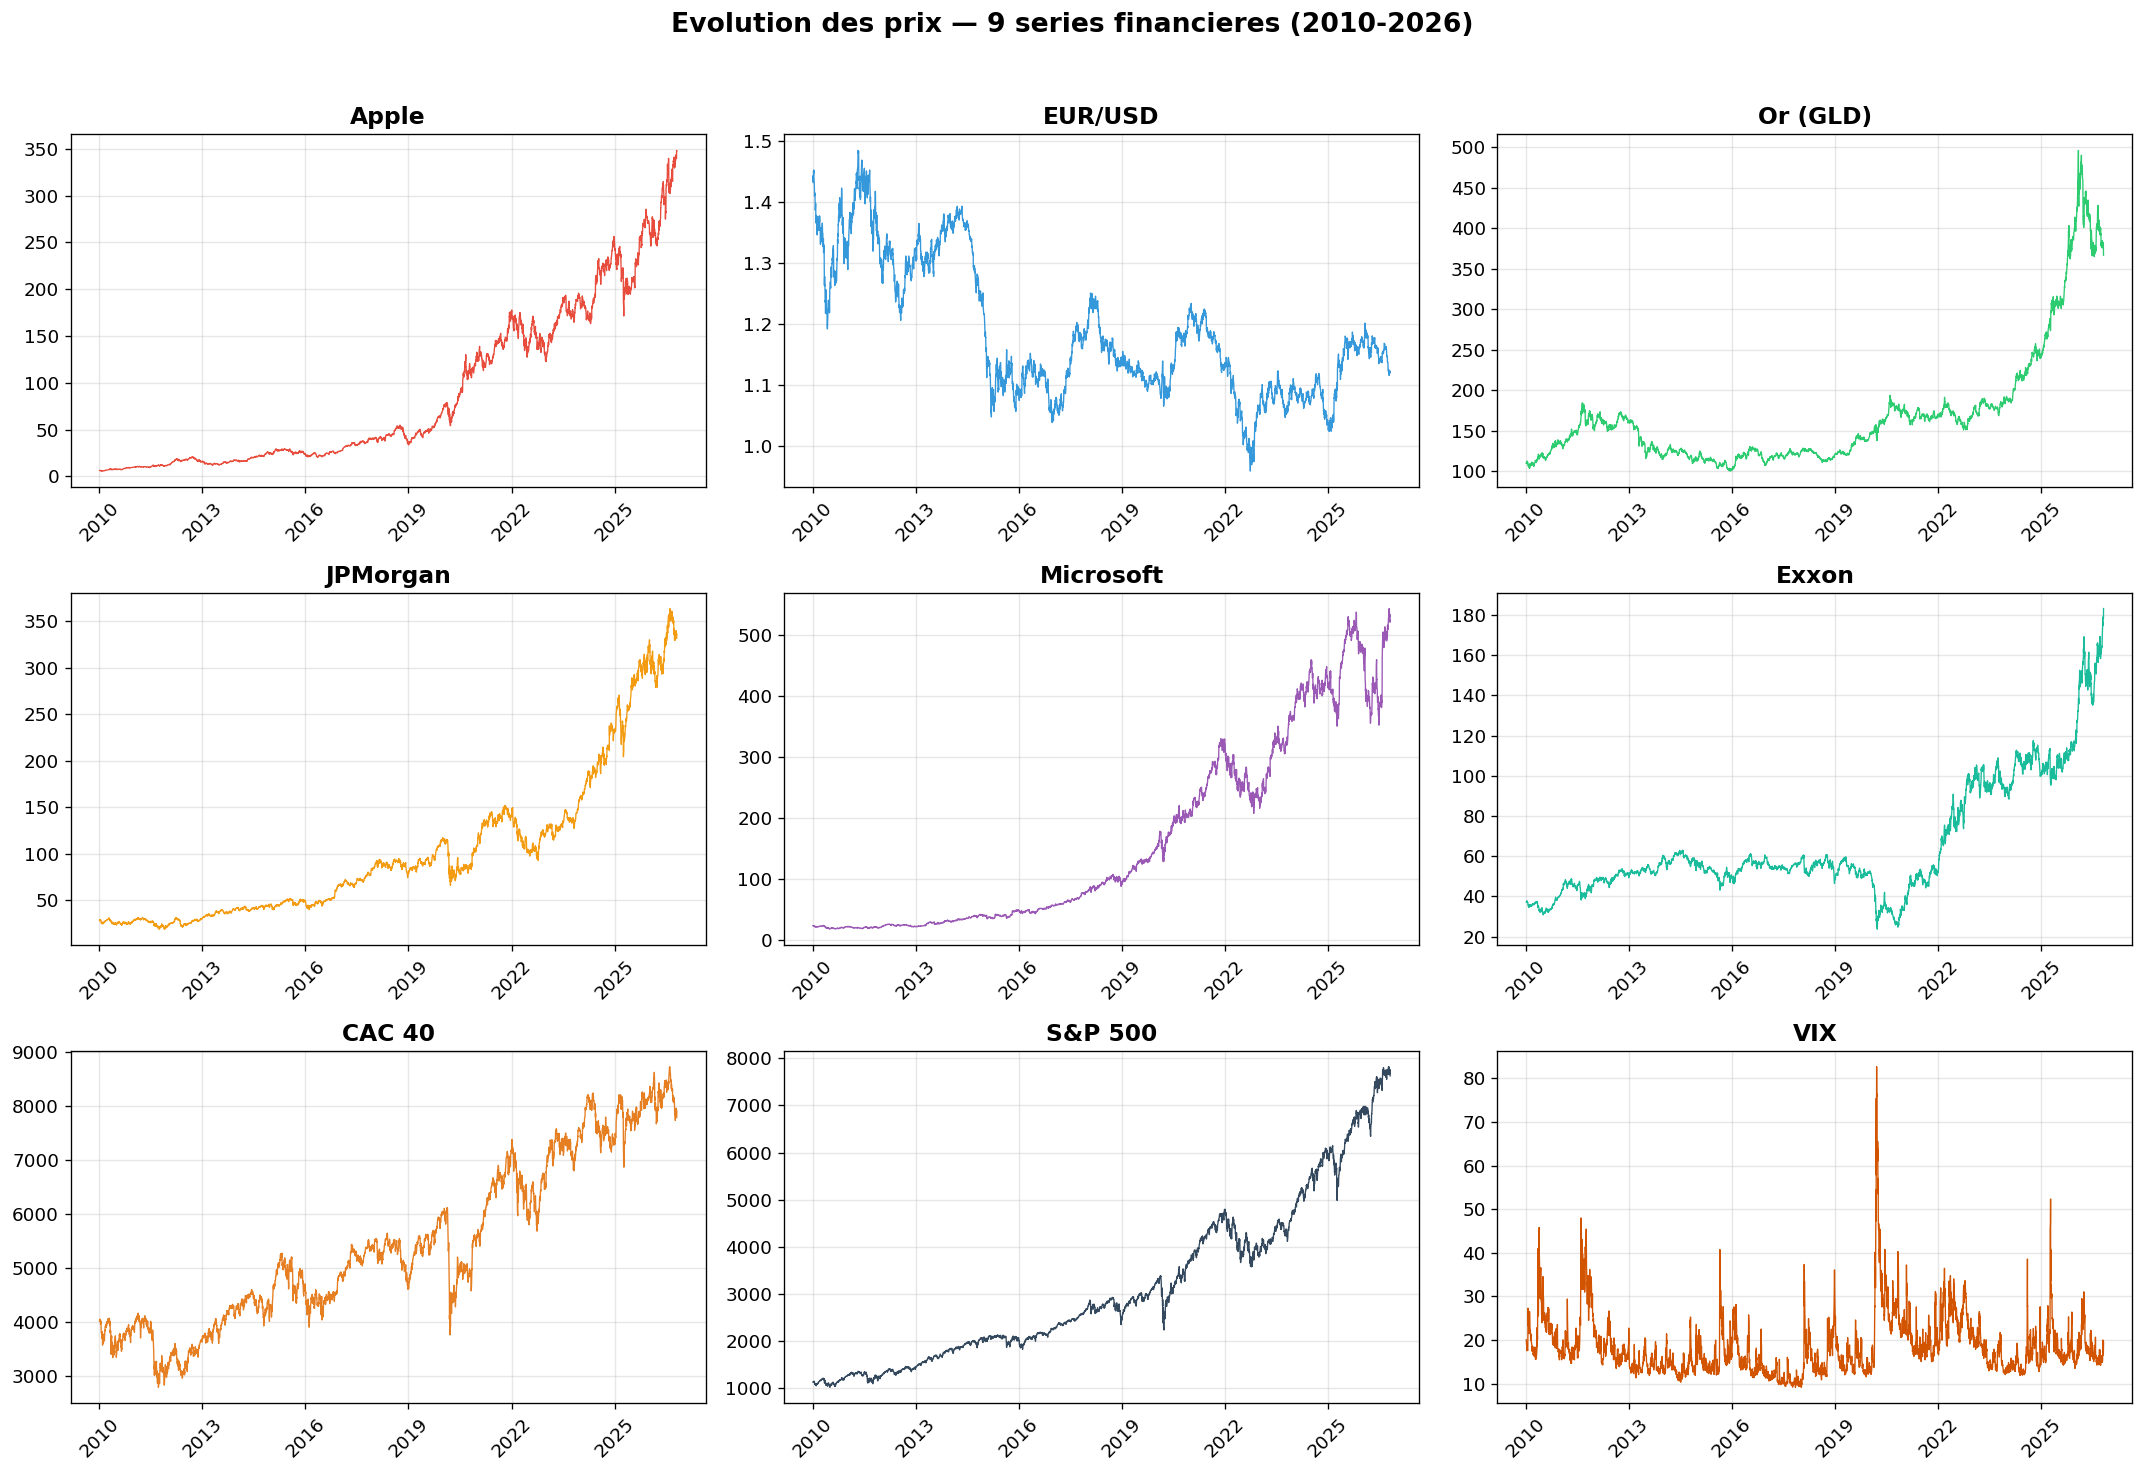
\includegraphics[width=0.95\linewidth]{02_evolution_prix_9series.png}
\caption{\'Evolution des prix des 9 s\'eries Yahoo Finance (2010--2026)}
\label{fig:prix_yahoo}
\end{figure}

\begin{figure}[H]
\centering
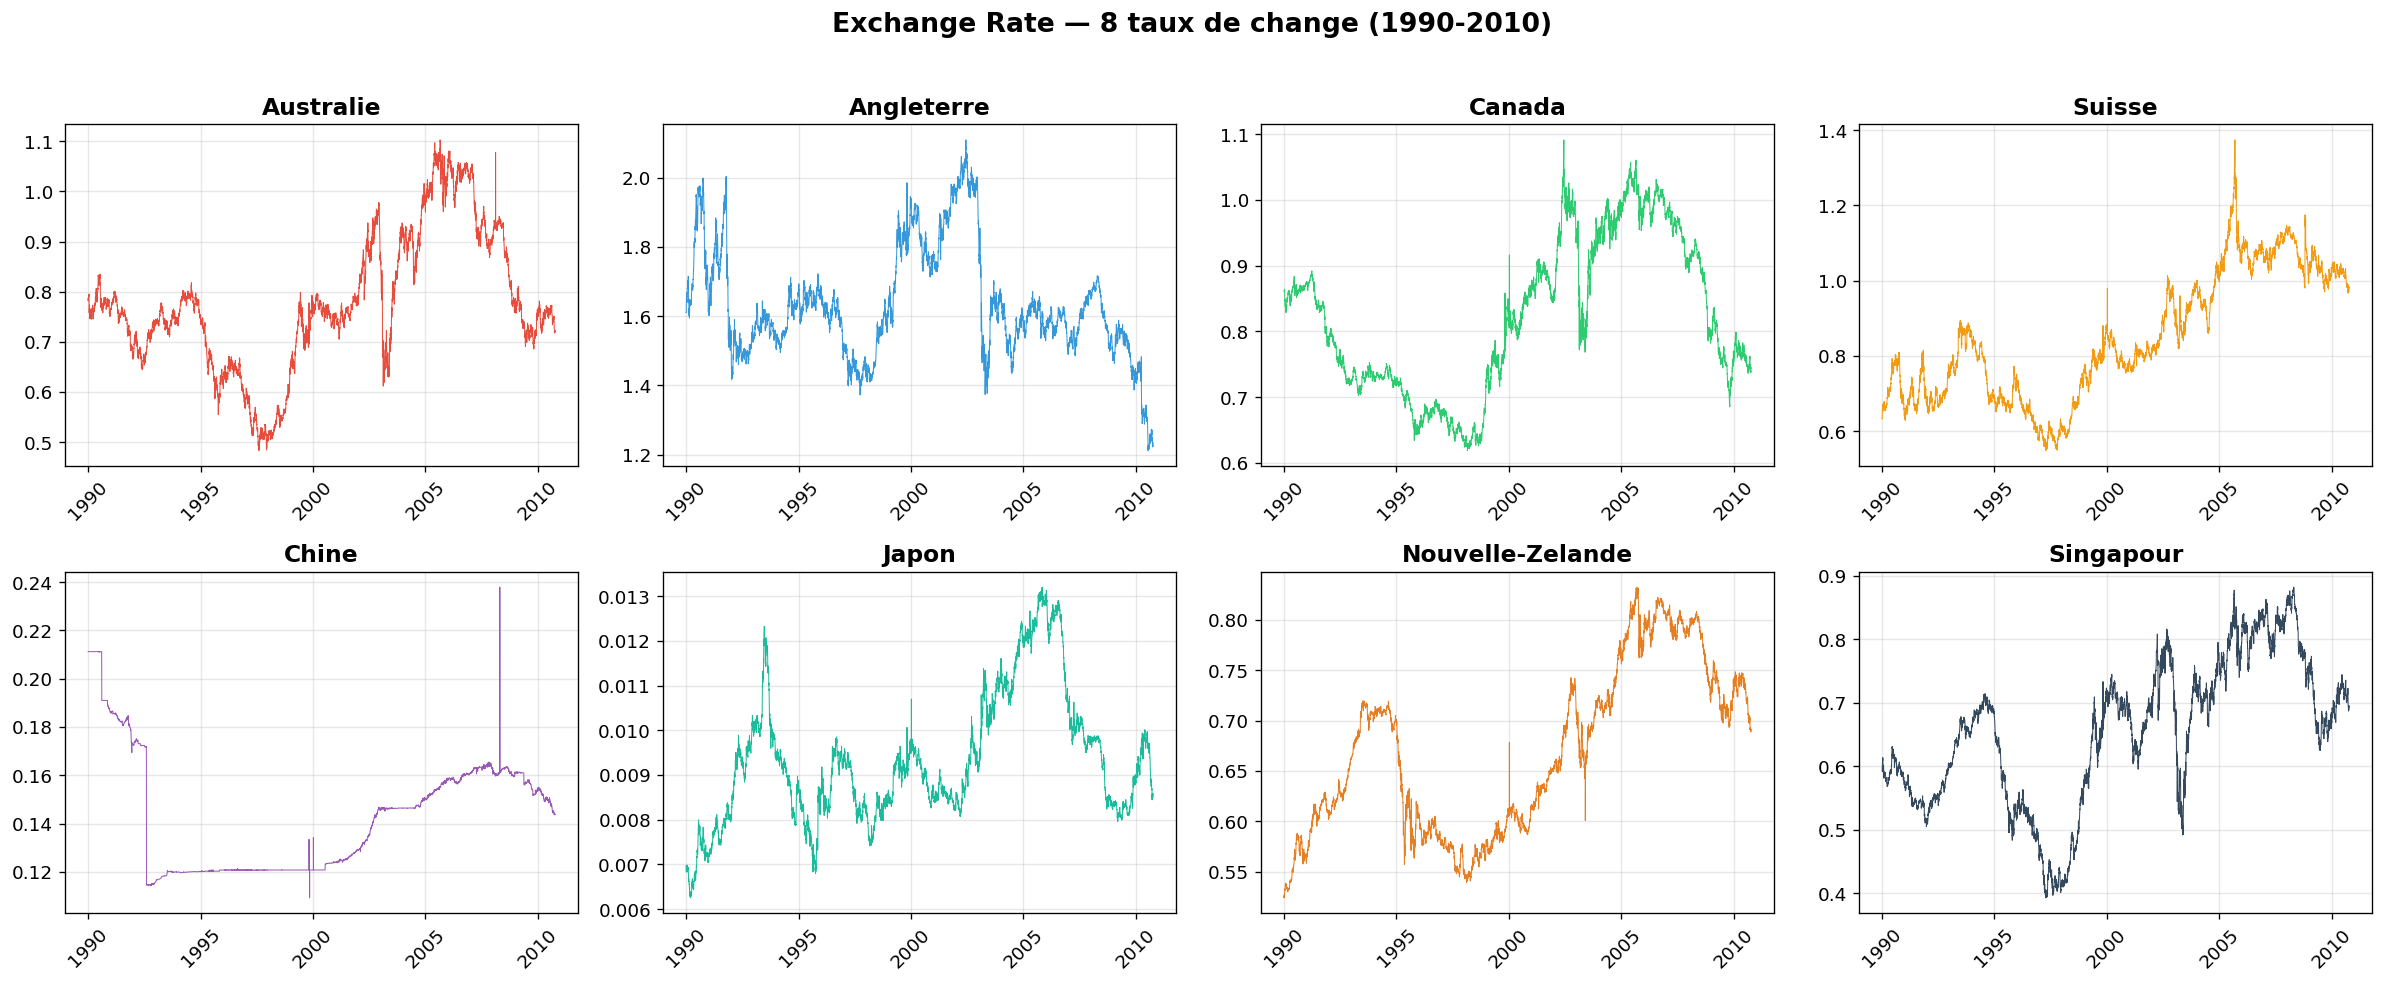
\includegraphics[width=0.95\linewidth]{10_exchange_rate_series.png}
\caption{\'Evolution des 8 taux de change (Exchange Rate, 1990--2010)}
\label{fig:exchange_series}
\end{figure}

\begin{figure}[H]
\centering
\begin{subfigure}[b]{0.48\linewidth}
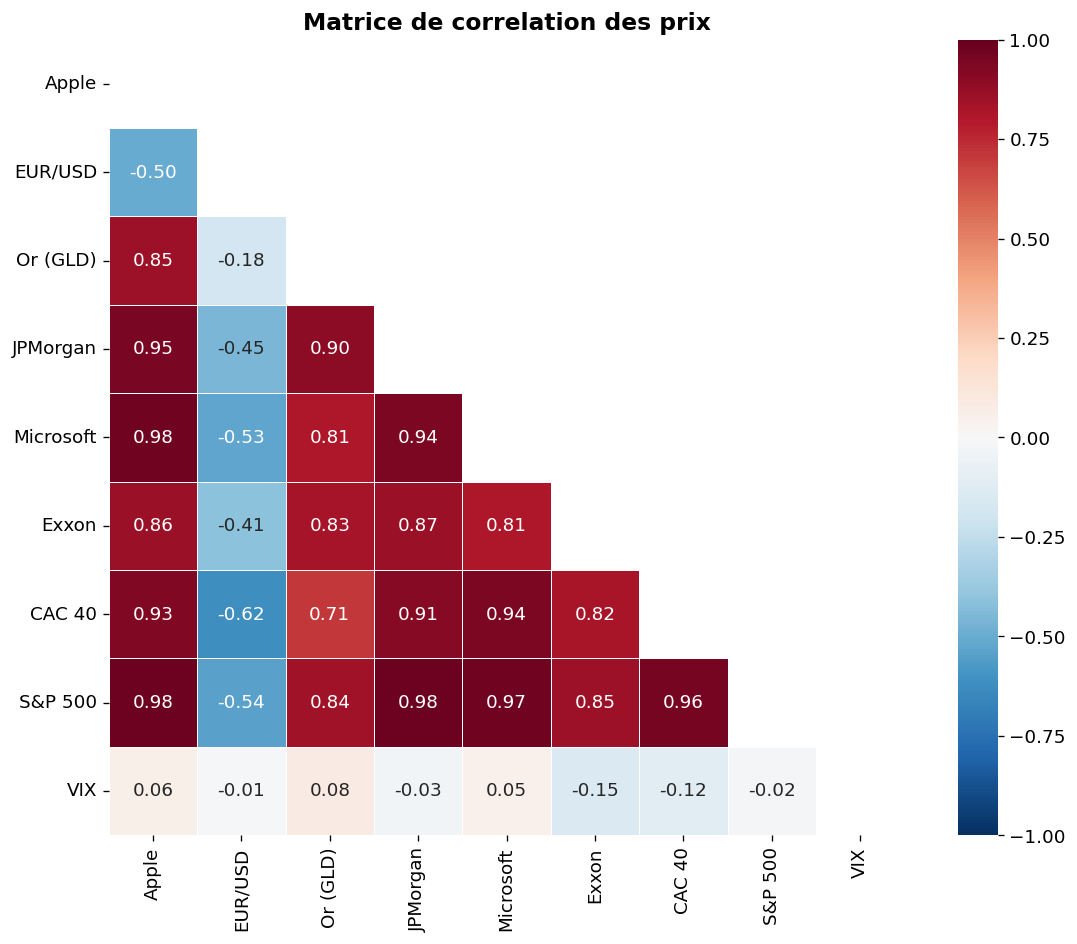
\includegraphics[width=\linewidth]{04_correlation_prix.png}
\caption{Corr\'elation prix Yahoo}
\end{subfigure}
\hfill
\begin{subfigure}[b]{0.48\linewidth}
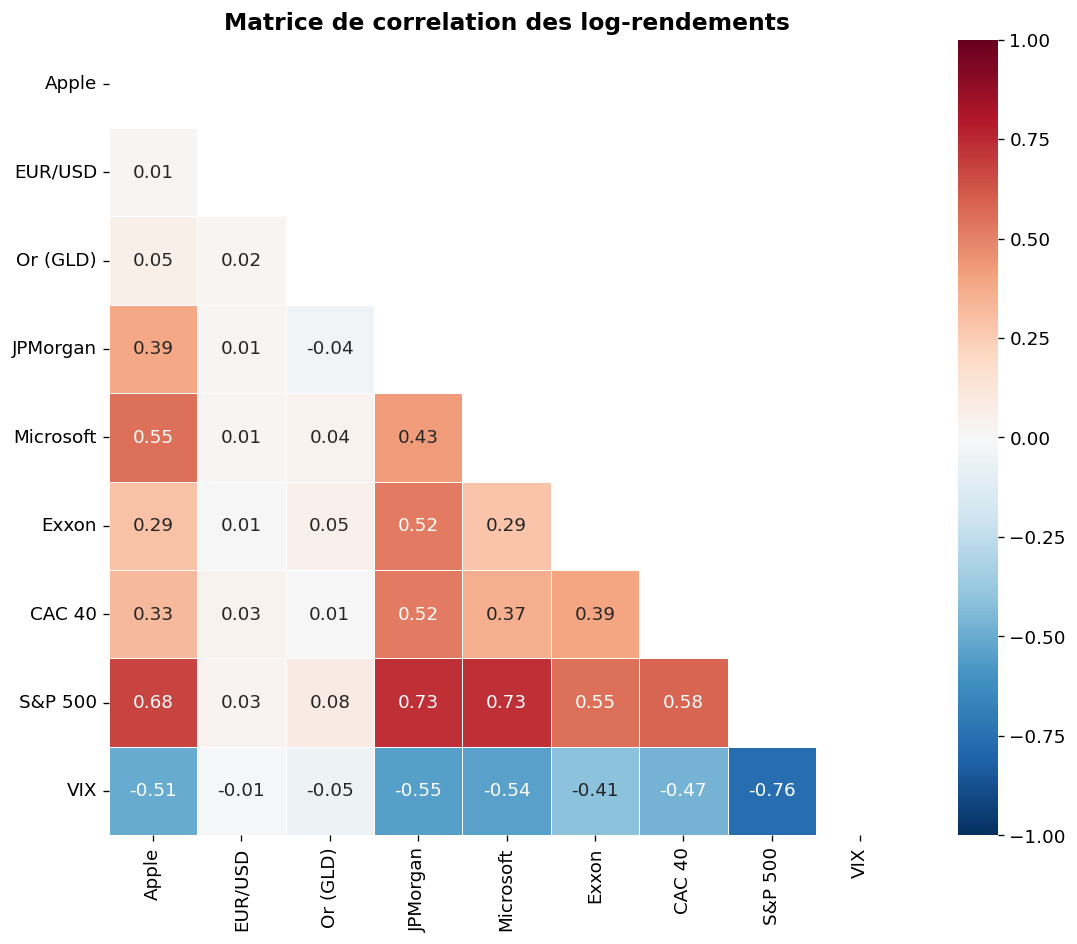
\includegraphics[width=\linewidth]{07_correlation_log_rendements.png}
\caption{Corr\'elation log-rendements Yahoo}
\end{subfigure}
\caption{Matrices de corr\'elation --- prix bruts vs.\ log-rendements}
\label{fig:correlations}
\end{figure}

\subsection{D\'ecoupage temporel}

\begin{table}[H]
\centering
\caption{D\'ecoupage temporel (sans fuite de donn\'ees)}
\begin{tabular}{lccc}
\toprule
\textbf{Dataset} & \textbf{Train} & \textbf{Validation} & \textbf{Test} \\
\midrule
Yahoo Finance & 2010--2020 (2\,734 j.) & 2021--2022 (501 j.) & 2023--2026 (945 j.) \\
Exchange Rate & 80\% (6\,070 j.) & 10\% (759 j.) & 10\% (759 j.) \\
\bottomrule
\end{tabular}
\end{table}

\begin{figure}[H]
\centering
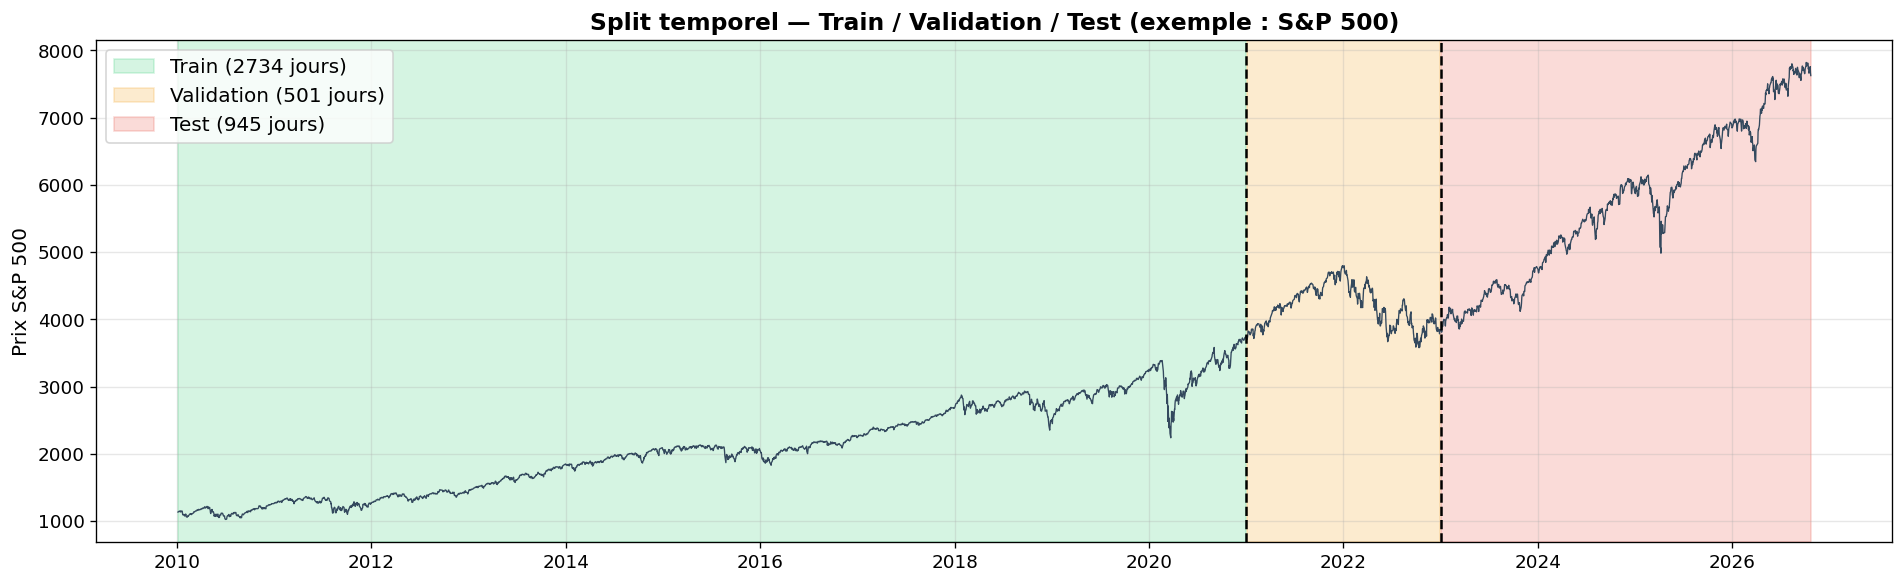
\includegraphics[width=0.95\linewidth]{08_split_temporel.png}
\caption{D\'ecoupage temporel train/validation/test --- Yahoo Finance}
\label{fig:split}
\end{figure}

\begin{figure}[H]
\centering
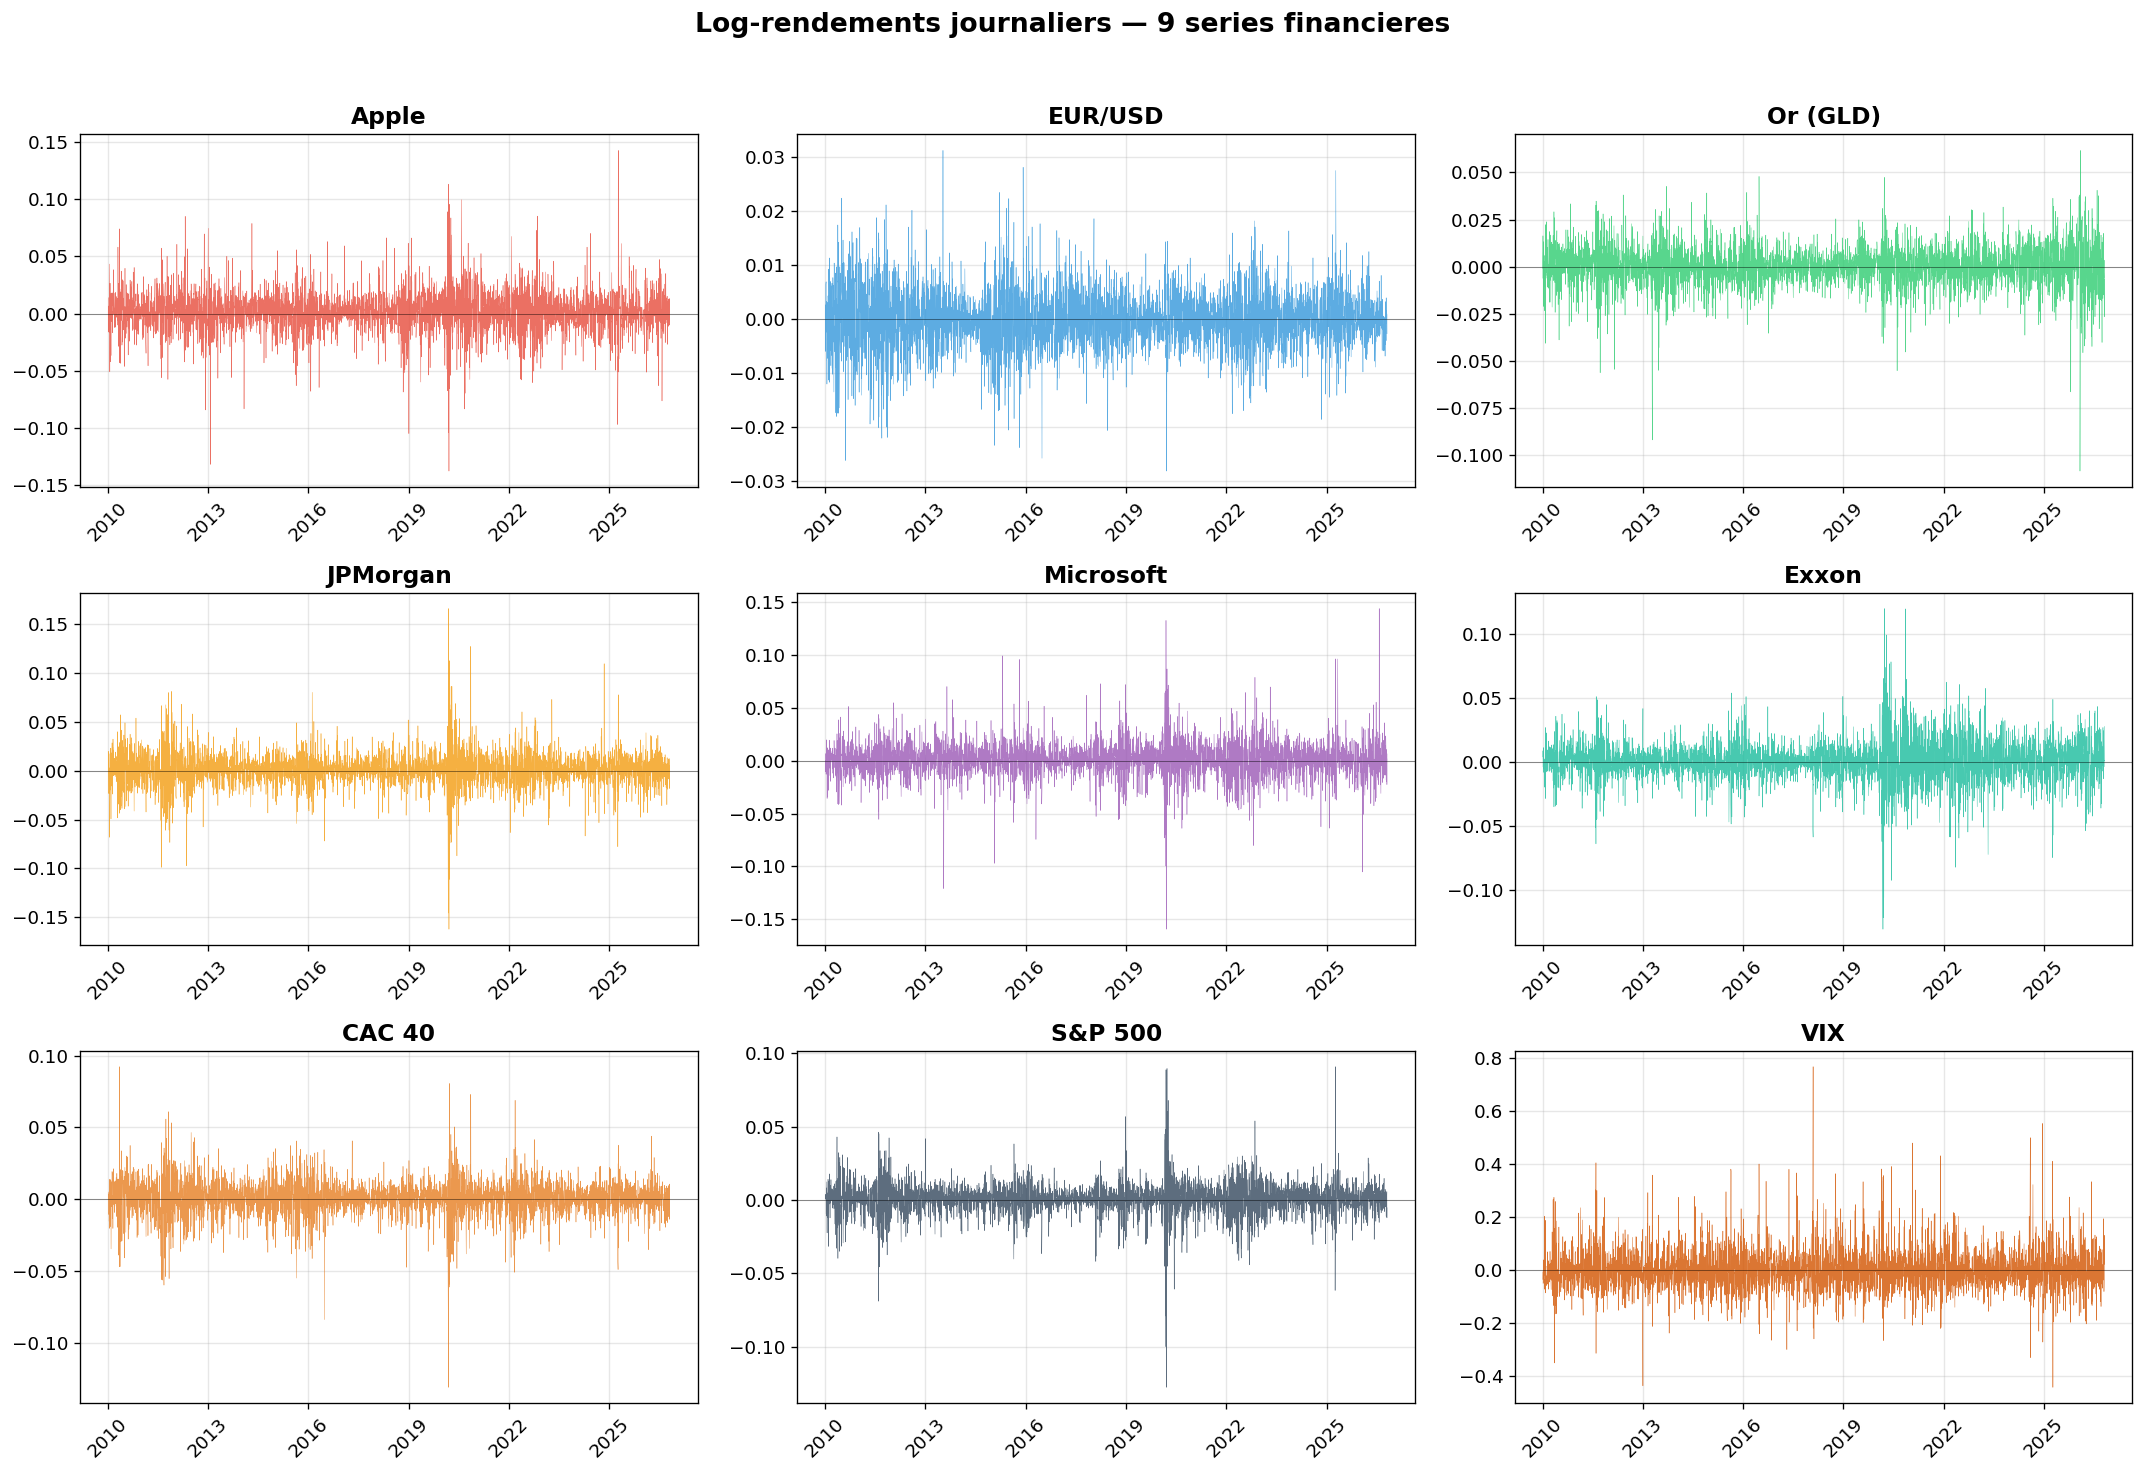
\includegraphics[width=0.95\linewidth]{05_log_rendements_9series.png}
\caption{Log-rendements des 9 s\'eries Yahoo Finance}
\label{fig:log_rendements}
\end{figure}

\begin{figure}[H]
\centering
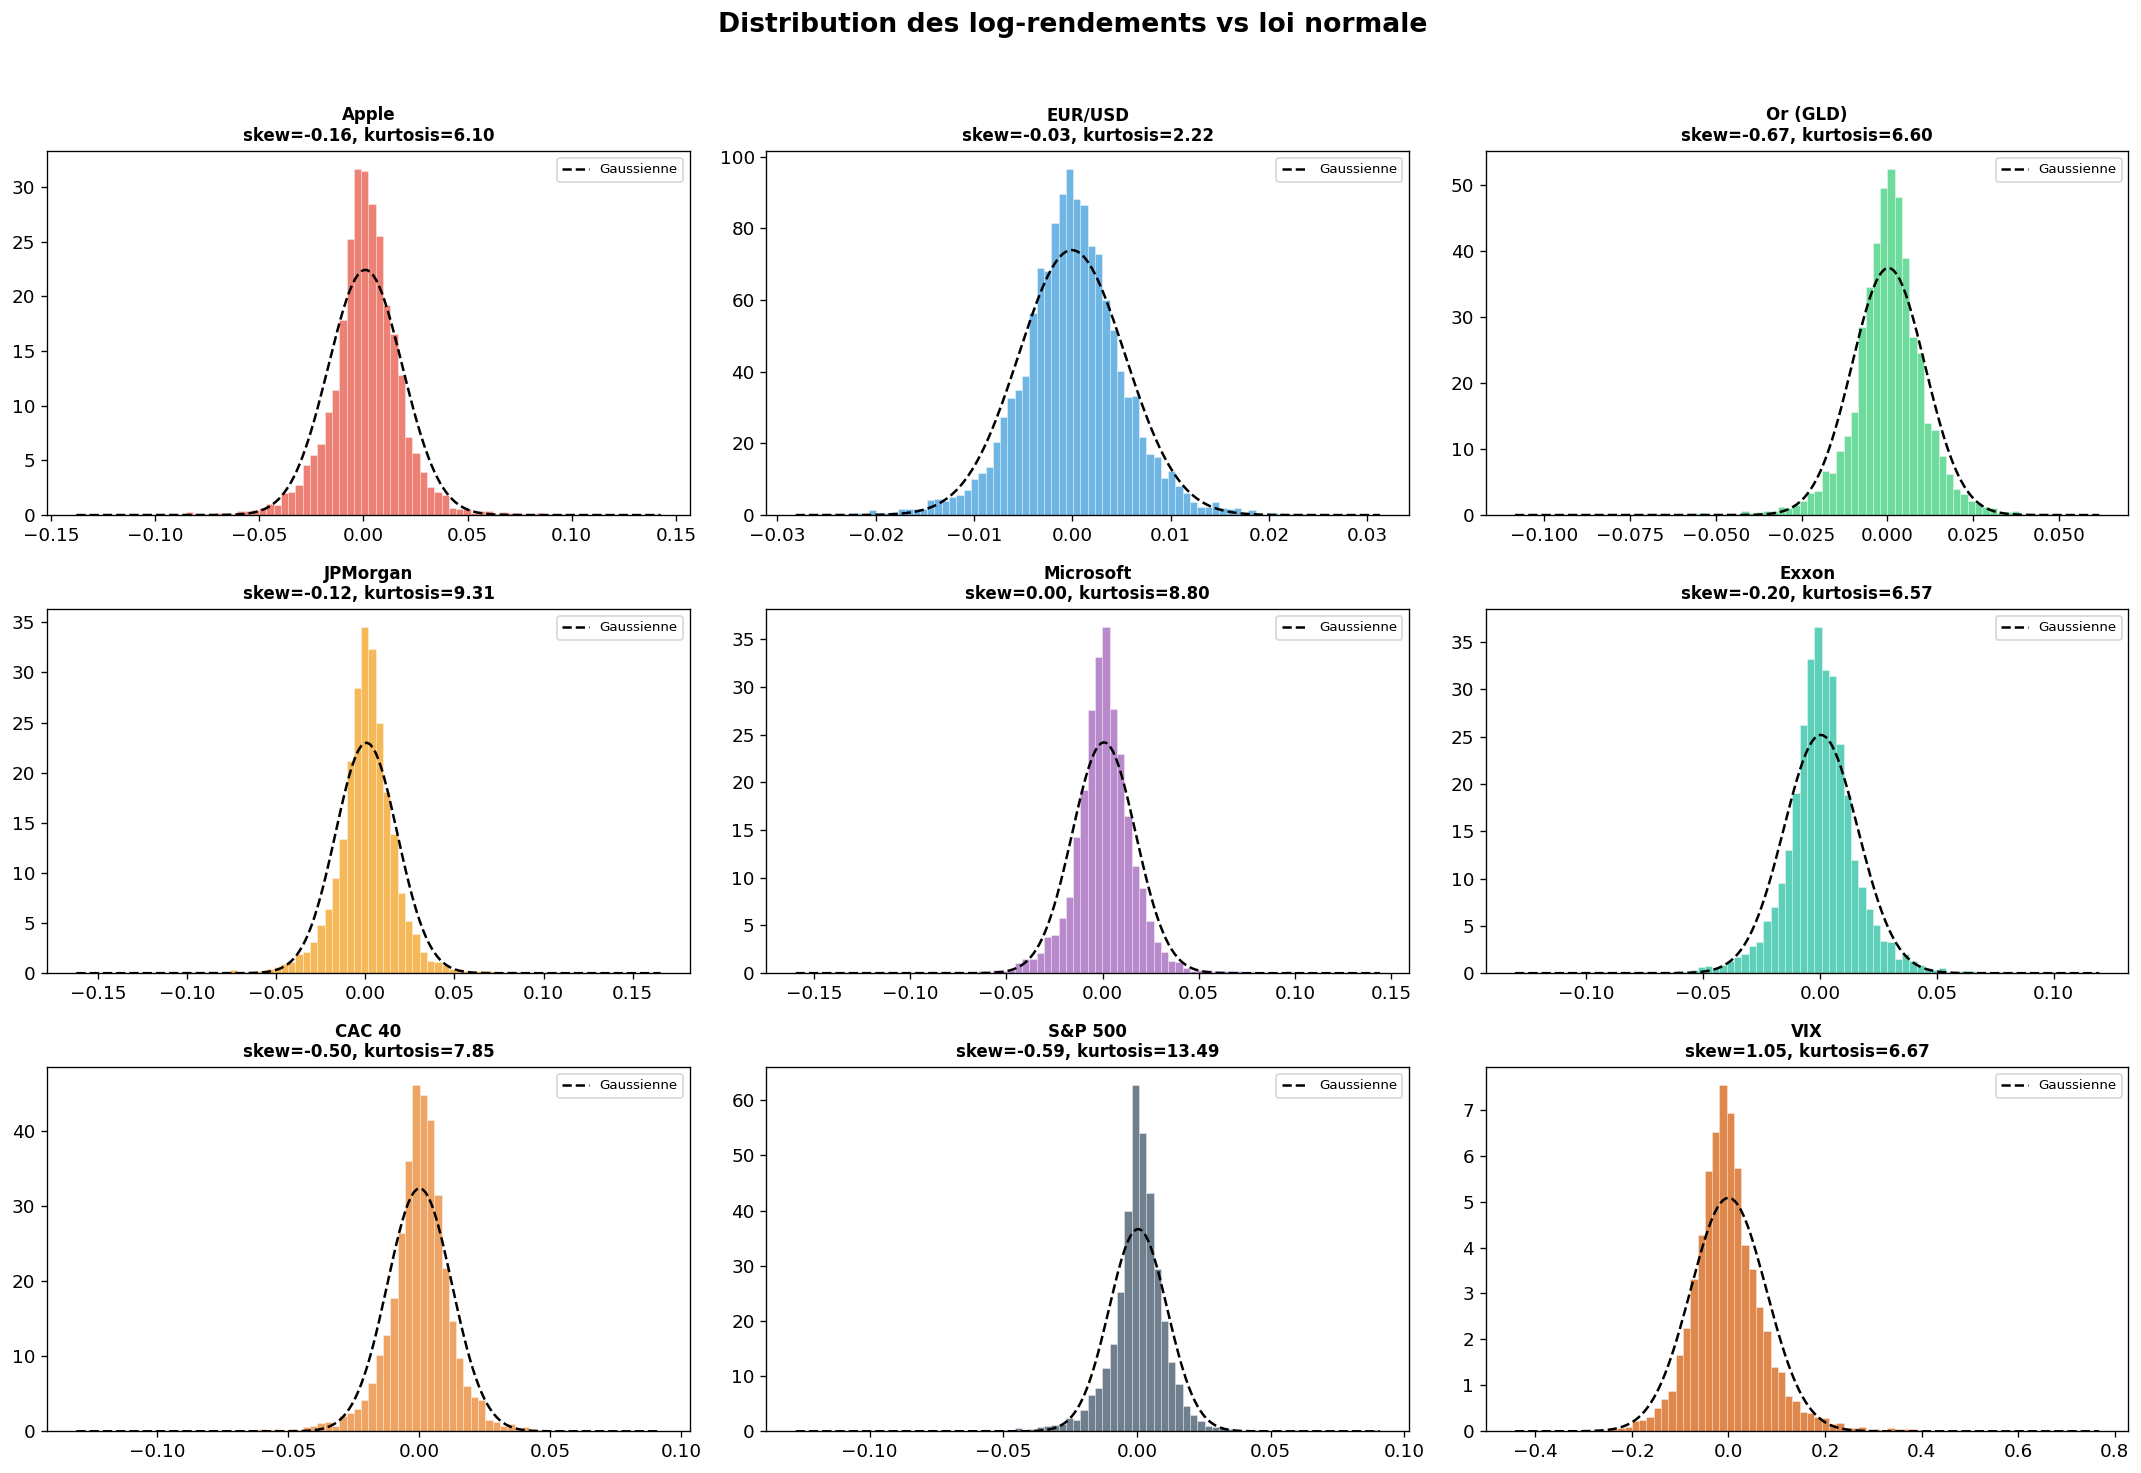
\includegraphics[width=0.95\linewidth]{06_distribution_log_rendements.png}
\caption{Distribution des log-rendements (histogrammes)}
\label{fig:distribution_lr}
\end{figure}

\subsection{Protocole exp\'erimental}

\begin{enumerate}
    \item \textbf{Pr\'etraitement} : calcul des log-rendements, standardisation sur train
    \item \textbf{Baselines} : entra\^inement sur train, s\'election d'hyperparamètres sur validation, \'evaluation sur test
    \item \textbf{CSDI} : entra\^inement (100 \'epoques, batch=16, lr=$10^{-3}$), \'evaluation sur test avec 6 configurations de masquage ($\{10\%, 30\%, 50\%\} \times \{\text{al\'eatoire, bloc}\}$)
    \item \textbf{SHAP} : analyse sur XGBoost et LightGBM pour la pr\'ediction du S\&P 500
    \item \textbf{Test DM} : comparaison statistique de toutes les paires de baselines
\end{enumerate}

% ══════════════════════════════════════════════════════════
% 4. RESULTATS
% ══════════════════════════════════════════════════════════
\section{R\'esultats}

\subsection{Baselines --- Pr\'evision (Yahoo Finance)}

\begin{table}[H]
\centering
\caption{Performance des baselines (lookback=20, horizon=5, log-rendements normalis\'es)}
\begin{tabular}{lcc}
\toprule
\textbf{Mod\`ele} & \textbf{MAE} & \textbf{RMSE} \\
\midrule
\textbf{Zero} & \textbf{0.6503} & \textbf{0.9280} \\
LightGBM & 0.6628 & 0.9398 \\
XGBoost & 0.6639 & 0.9421 \\
LSTM & 0.6667 & 0.9470 \\
ARIMA(1,0,0) & 0.6776 & 0.9639 \\
Na\"if & 0.9440 & 1.3197 \\
\bottomrule
\end{tabular}
\end{table}

\textbf{Observations :} Le baseline z\'ero (pr\'edire toujours 0, la moyenne des log-rendements normalis\'es) obtient le meilleur MAE (0.6503), devant LightGBM (0.6628) et XGBoost (0.6639). Aucun mod\`ele appris ne bat le z\'ero (LightGBM : $+1.9\%$ de MAE, XGBoost : $+2.1\%$). Le baseline na\"if est nettement inf\'erieur.

\begin{remarque}[Interpr\'etation du baseline z\'ero]
Ce r\'esultat est attendu pour des log-rendements normalis\'es de s\'eries financi\`eres quasi-stationnaires. Pr\'edire la moyenne (ici z\'ero apr\`es standardisation) est l'estimateur optimal au sens du MSE lorsque les rendements sont approximativement un bruit blanc. La valeur ajout\'ee potentielle des mod\`eles ML r\'esiderait dans la \textbf{quantification de l'incertitude} (r\'egression quantile, intervalles CSDI), mais nos r\'esultats ne d\'emontrent pas d'am\'elioration en pr\'evision ponctuelle sur ce jeu de donn\'ees.
\end{remarque}

\begin{figure}[H]
\centering
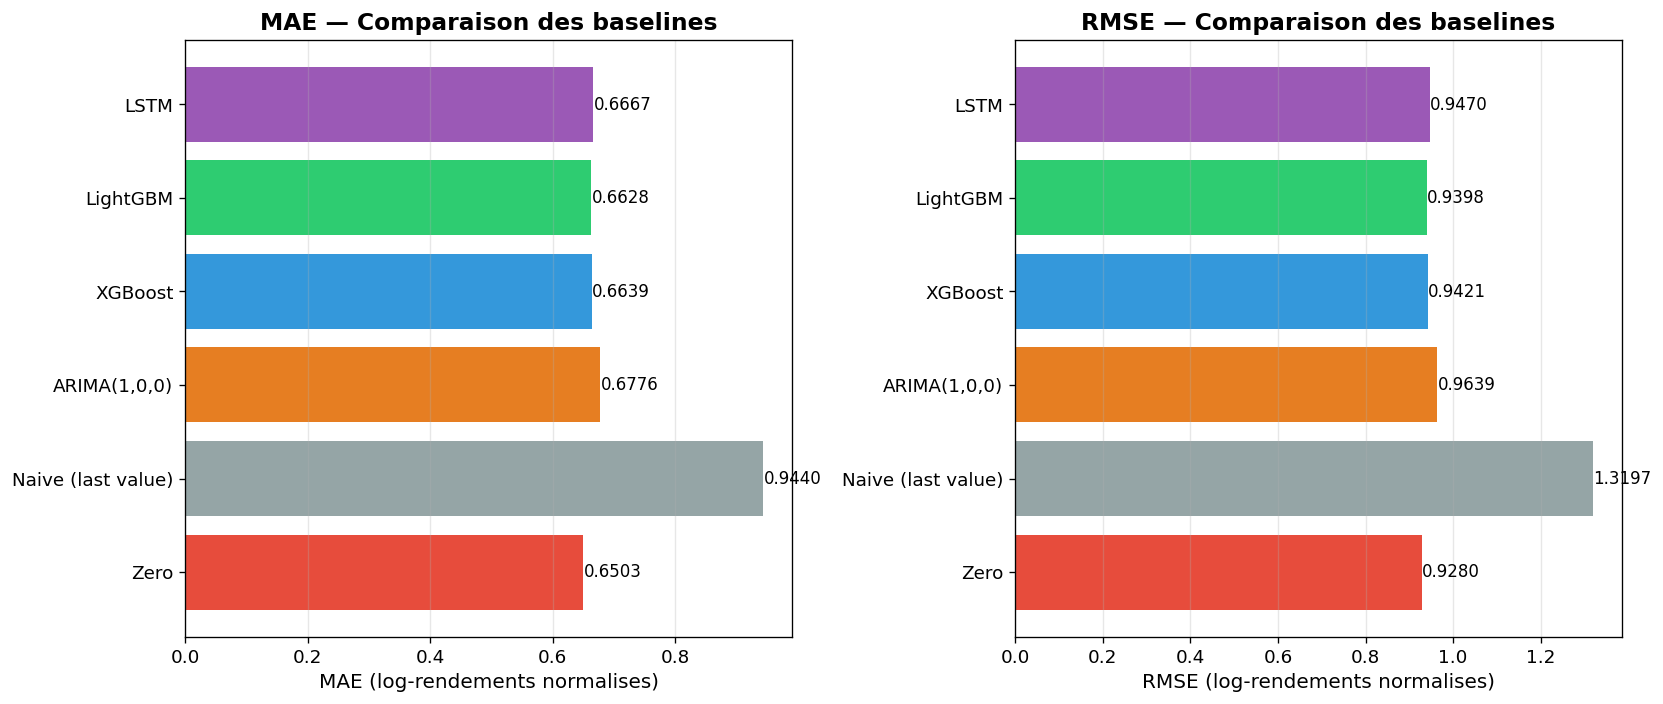
\includegraphics[width=0.95\linewidth]{16_baselines_comparaison.png}
\caption{Comparaison des baselines --- MAE et RMSE par mod\`ele}
\label{fig:baselines_comp}
\end{figure}

\begin{figure}[H]
\centering
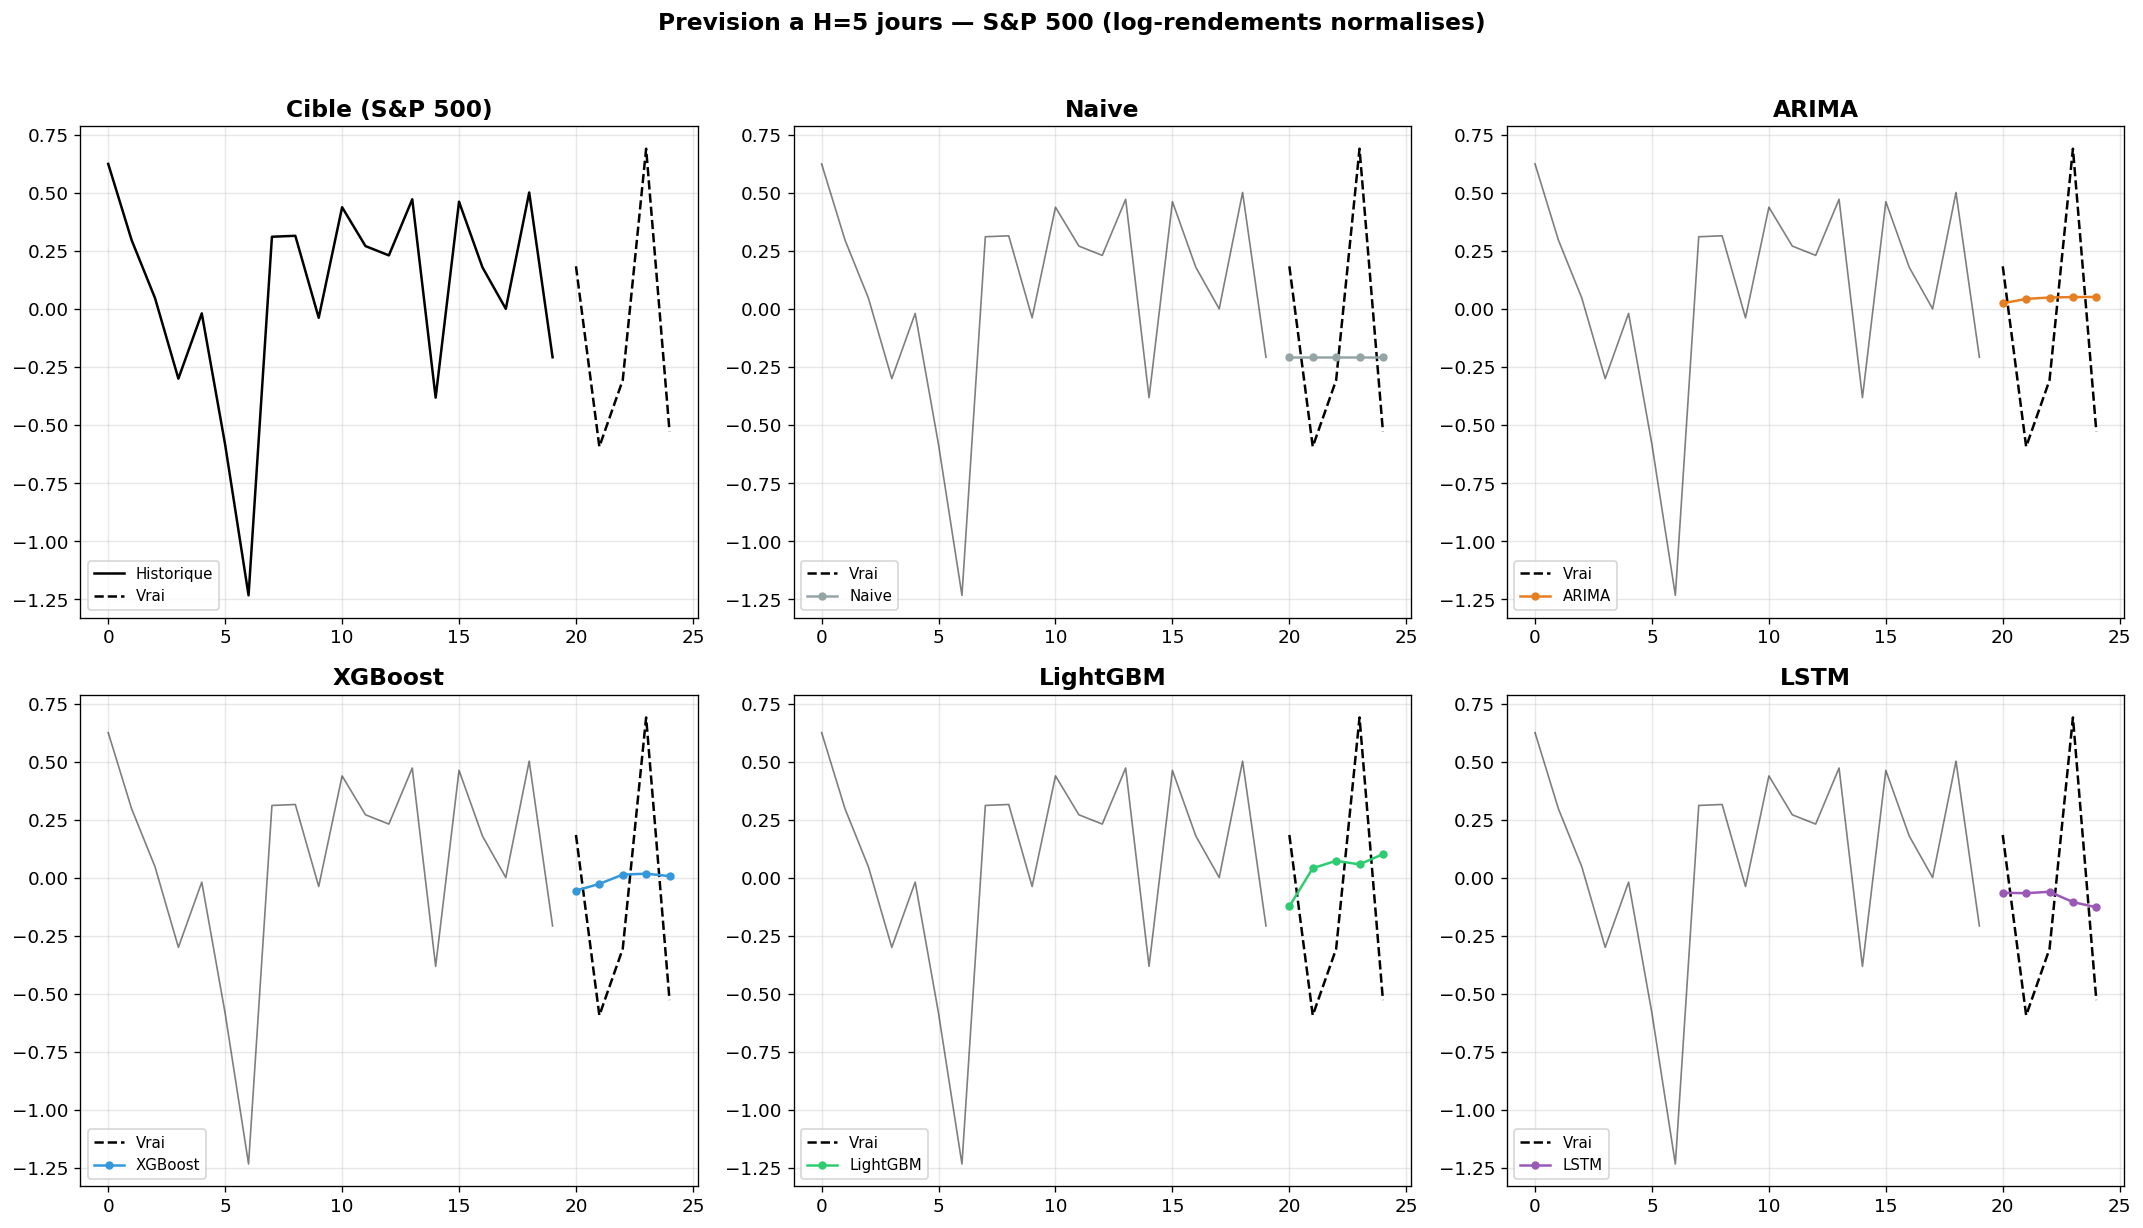
\includegraphics[width=0.95\linewidth]{17_baselines_exemple_prevision.png}
\caption{Exemple de pr\'evision sur 5 jours (test set)}
\label{fig:baselines_exemple}
\end{figure}

\subsection{CSDI --- Imputation (Exchange Rate)}

\begin{table}[H]
\centering
\caption{CSDI Imputation --- Exchange Rate (8 devises)}
\begin{tabular}{lccc}
\toprule
\textbf{Configuration} & \textbf{RMSE} & \textbf{MAE} & \textbf{CRPS} \\
\midrule
10\% al\'eatoire & 0.0030 & 0.0017 & 0.0019 \\
10\% bloc & 0.0073 & 0.0045 & 0.0051 \\
30\% al\'eatoire & 0.0035 & 0.0019 & 0.0022 \\
30\% bloc & 0.0126 & 0.0078 & 0.0088 \\
50\% al\'eatoire & 0.0041 & 0.0023 & 0.0026 \\
50\% bloc & 0.0154 & 0.0096 & 0.0107 \\
\bottomrule
\end{tabular}
\end{table}

\begin{figure}[H]
\centering
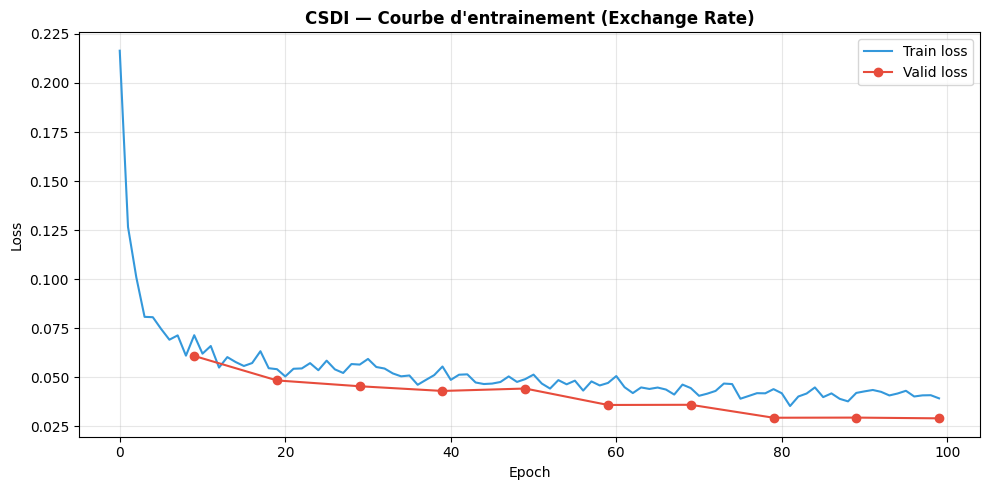
\includegraphics[width=0.85\linewidth]{14_csdi_training_loss.png}
\caption{Courbe d'entra\^inement CSDI --- Exchange Rate (100 \'epoques)}
\label{fig:csdi_loss_er}
\end{figure}

\begin{figure}[H]
\centering
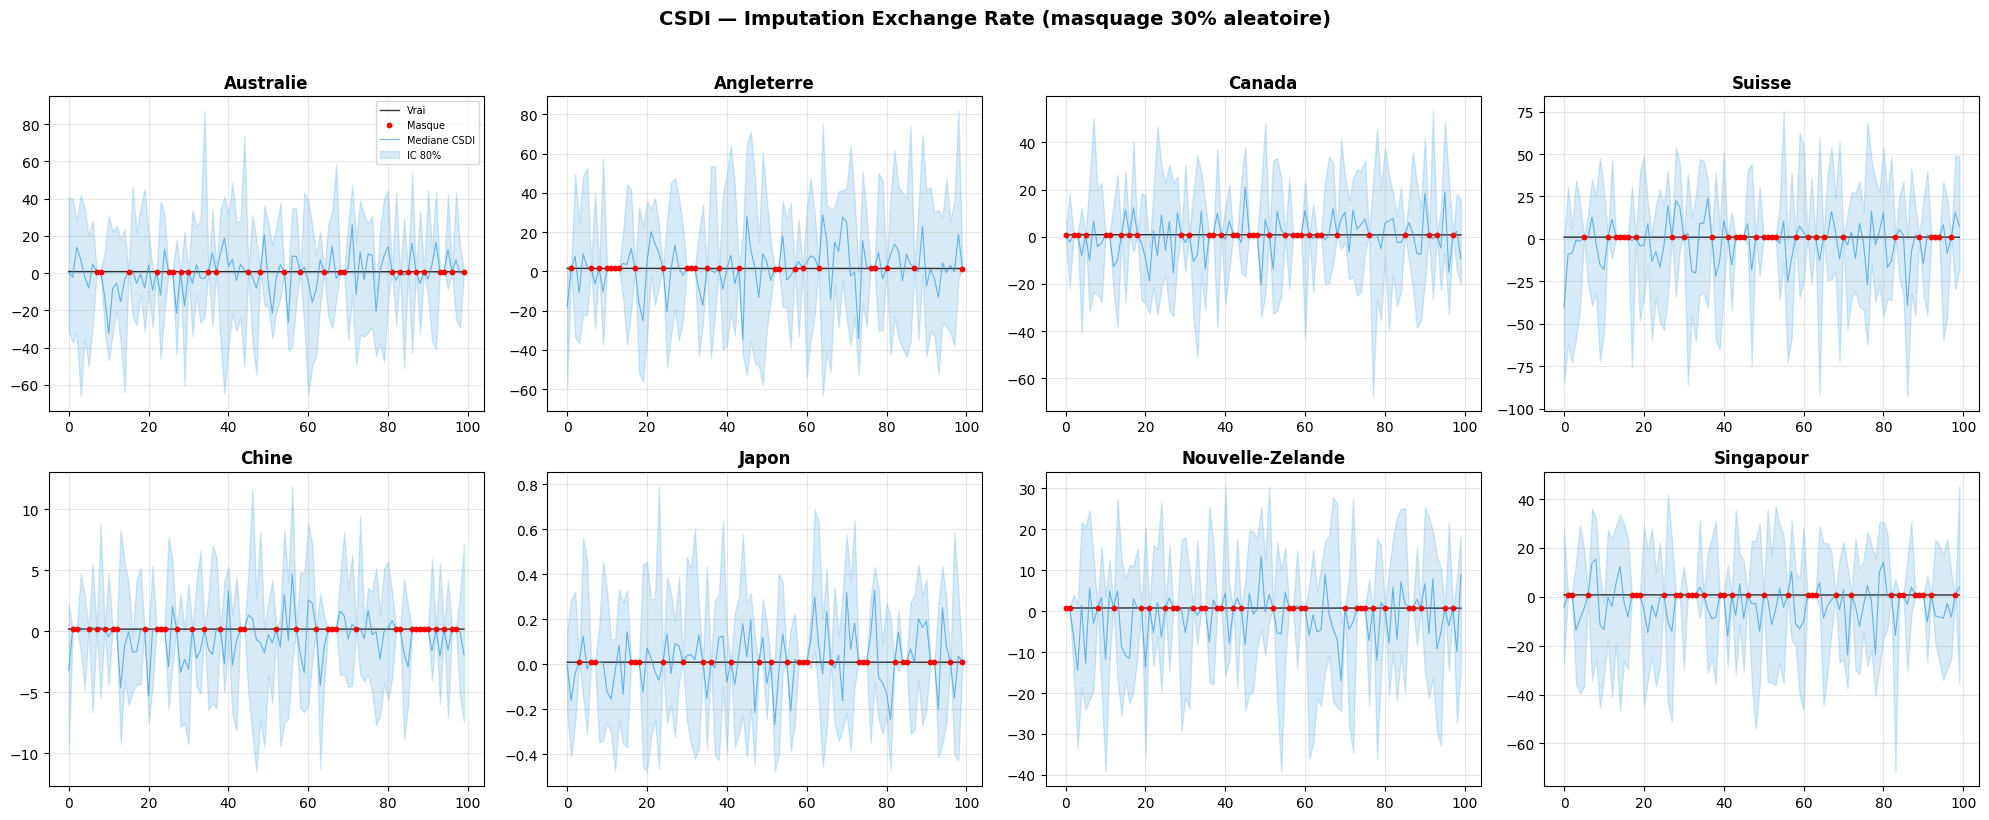
\includegraphics[width=0.95\linewidth]{15_csdi_imputation_exemple.png}
\caption{Imputation CSDI --- Exchange Rate : valeurs r\'eelles, masqu\'ees, imput\'ees avec IC \`a 80\%}
\label{fig:csdi_imputation_er}
\end{figure}

\begin{remarque}[Largeur des intervalles de confiance]
Les IC \`a 80\% affich\'es sur les figures~\ref{fig:csdi_imputation_er} et~\ref{fig:csdi_imputation_yahoo} apparaissent tr\`es larges, notamment pour les configurations de masquage bloc \`a 50\%. Cela refl\`ete la forte incertitude inh\'erente \`a l'imputation de longues s\'equences contigu\"es de donn\'ees financi\`eres volatiles. \textbf{Limite :} nous ne calculons pas la couverture empirique (proportion des vraies valeurs tombant dans l'IC) ni la largeur moyenne, qui seraient n\'ecessaires pour \'evaluer rigoureusement la calibration. Un IC nominalement \`a 80\% pourrait couvrir bien plus (ou moins) de 80\% des valeurs r\'eelles.
\end{remarque}

\subsection{CSDI --- Imputation (Yahoo Finance)}

\begin{table}[H]
\centering
\caption{CSDI Imputation --- Yahoo Finance (9 s\'eries)}
\begin{tabular}{lccc}
\toprule
\textbf{Configuration} & \textbf{RMSE} & \textbf{MAE} & \textbf{CRPS} \\
\midrule
10\% al\'eatoire & 0.0198 & 0.0110 & 0.0076 \\
10\% bloc & 0.0276 & 0.0140 & 0.0101 \\
30\% al\'eatoire & 0.0205 & 0.0113 & 0.0078 \\
30\% bloc & 0.0280 & 0.0142 & 0.0103 \\
50\% al\'eatoire & 0.0220 & 0.0118 & 0.0083 \\
50\% bloc & 0.0284 & 0.0142 & 0.0103 \\
\bottomrule
\end{tabular}
\end{table}

\textbf{Observations :}
\begin{itemize}
    \item Le masquage bloc est syst\'ematiquement plus difficile que le masquage al\'eatoire (l'interpolation lin\'eaire est moins efficace sans voisins proches)
    \item La performance se d\'egrade avec le taux de masquage, surtout en mode bloc
    \item Le CRPS est inf\'erieur au MAE par construction math\'ematique (le second terme de l'\'equation~\eqref{eq:crps} est toujours positif), ce qui ne constitue \textbf{pas} une preuve de bonne calibration. La \textbf{couverture empirique} des IC \`a 80\% (proportion des vraies valeurs dans $[q_{10}, q_{90}]$) a \'et\'e mesur\'ee : elle varie de 50\% \`a 61\% selon la configuration (Table~\ref{tab:coverage}), loin de la cible de 80\%, indiquant un mod\`ele \textbf{sous-dispersif} dont les intervalles sont trop \'etroits
    \item Ces r\'esultats doivent \^etre compar\'es aux baselines d'imputation (z\'ero et interpolation lin\'eaire) --- voir Table~\ref{tab:imputation_baselines}
\end{itemize}

\begin{table}[H]
\centering
\caption{Couverture empirique des IC \`a 80\% (cible : 80\%) et largeur moyenne}
\label{tab:coverage}
\begin{tabular}{llcc}
\toprule
\textbf{Dataset} & \textbf{Masquage} & \textbf{Couverture (\%)} & \textbf{Largeur IC} \\
\midrule
\multirow{6}{*}{Exchange Rate}
 & 10\% al\'eatoire & 57.1 & 0.0034 \\
 & 30\% al\'eatoire & 56.5 & 0.0038 \\
 & 50\% al\'eatoire & 54.3 & 0.0046 \\
 & 10\% bloc & 52.8 & 0.0082 \\
 & 30\% bloc & 50.4 & 0.0136 \\
 & 50\% bloc & 54.3 & 0.0182 \\
\midrule
\multirow{6}{*}{Yahoo Finance}
 & 10\% al\'eatoire & 60.6 & 0.0233 \\
 & 30\% al\'eatoire & 59.3 & 0.0234 \\
 & 50\% al\'eatoire & 57.8 & 0.0237 \\
 & 10\% bloc & 57.0 & 0.0253 \\
 & 30\% bloc & 55.2 & 0.0246 \\
 & 50\% bloc & 54.3 & 0.0240 \\
\bottomrule
\end{tabular}
\end{table}

La couverture moyenne est de $\sim$55\% (Exchange Rate) et $\sim$57\% (Yahoo), nettement inf\'erieure \`a la cible de 80\%. CSDI est donc \textbf{sous-dispersif} : les 10 trajectoires \'echantillonn\'ees ne couvrent pas suffisamment la variabilit\'e r\'eelle. Ce ph\'enom\`ene est classique pour un nombre limit\'e d'\'echantillons et pourrait s'am\'eliorer avec davantage de trajectoires (50 ou 100).

\begin{table}[H]
\centering
\caption{Baselines d'imputation --- Comparaison avec CSDI}
\label{tab:imputation_baselines}
\begin{tabular}{llcccccc}
\toprule
 & & \multicolumn{3}{c}{\textbf{Masquage al\'eatoire (RMSE)}} & \multicolumn{3}{c}{\textbf{Masquage bloc (RMSE)}} \\
\cmidrule(lr){3-5} \cmidrule(lr){6-8}
\textbf{Dataset} & \textbf{M\'ethode} & \textbf{10\%} & \textbf{30\%} & \textbf{50\%} & \textbf{10\%} & \textbf{30\%} & \textbf{50\%} \\
\midrule
\multirow{4}{*}{Exchange Rate}
  & Z\'ero & 0.1222 & 0.1228 & 0.1227 & 0.1226 & 0.1226 & 0.1227 \\
  & Interpolation & 0.0035 & 0.0040 & 0.0045 & \textbf{0.0062} & \textbf{0.0108} & \textbf{0.0133} \\
  & Gauss. cond.$^\dagger$ & 0.0802 & 0.0982 & 0.1149 & $\equiv$ z\'ero & $\equiv$ z\'ero & $\equiv$ z\'ero \\
  & \textbf{CSDI} & \textbf{0.0030} & \textbf{0.0035} & \textbf{0.0041} & 0.0073 & 0.0126 & 0.0154 \\
\midrule
\multirow{4}{*}{Yahoo Finance}
  & Z\'ero & 0.0268 & 0.0275 & 0.0277 & \textbf{0.0265} & \textbf{0.0269} & \textbf{0.0276} \\
  & Interpolation & 0.0341 & 0.0353 & 0.0356 & 0.0337 & 0.0347 & 0.0354 \\
  & \textbf{Gauss. cond.}$^\dagger$ & \textbf{0.0188} & \textbf{0.0199} & \textbf{0.0216} & $\equiv$ z\'ero & $\equiv$ z\'ero & $\equiv$ z\'ero \\
  & CSDI & 0.0198 & 0.0205 & 0.0220 & 0.0276 & 0.0280 & 0.0284 \\
\bottomrule
\multicolumn{8}{l}{\footnotesize $^\dagger$ En masquage bloc, toutes les s\'eries sont masqu\'ees simultan\'ement : la gaussienne d\'eg\'en\`ere en z\'ero.}
\end{tabular}
\end{table}

\begin{remarque}[Interpr\'etation des baselines]
Sur Exchange Rate (donn\'ees brutes normalis\'ees), CSDI bat toutes les baselines en masquage al\'eatoire (RMSE 0.0035 vs interpolation 0.0040) ; la gaussienne conditionnelle est peu performante ici (RMSE $>$ 0.08) car les taux de change non centr\'es sont mal approch\'es par la moyenne conditionnelle. En masquage bloc, l'interpolation reprend l'avantage (s\'eries lisses, voisins fiables). Sur Yahoo Finance (log-rendements centr\'es en 0), la gaussienne conditionnelle bat CSDI en masquage al\'eatoire (RMSE 0.0188 vs 0.0198 \`a 10\,\%) gr\^ace aux corr\'elations inter-s\'eries ; CSDI bat n\'eanmoins le z\'ero et l'interpolation. En masquage bloc, le z\'ero reprend l'avantage (RMSE 0.0265--0.0276 vs CSDI 0.0276--0.0284) ; la gaussienne d\'eg\'en\`ere en z\'ero car toutes les s\'eries sont masqu\'ees simultan\'ement.
\end{remarque}

\begin{figure}[H]
\centering
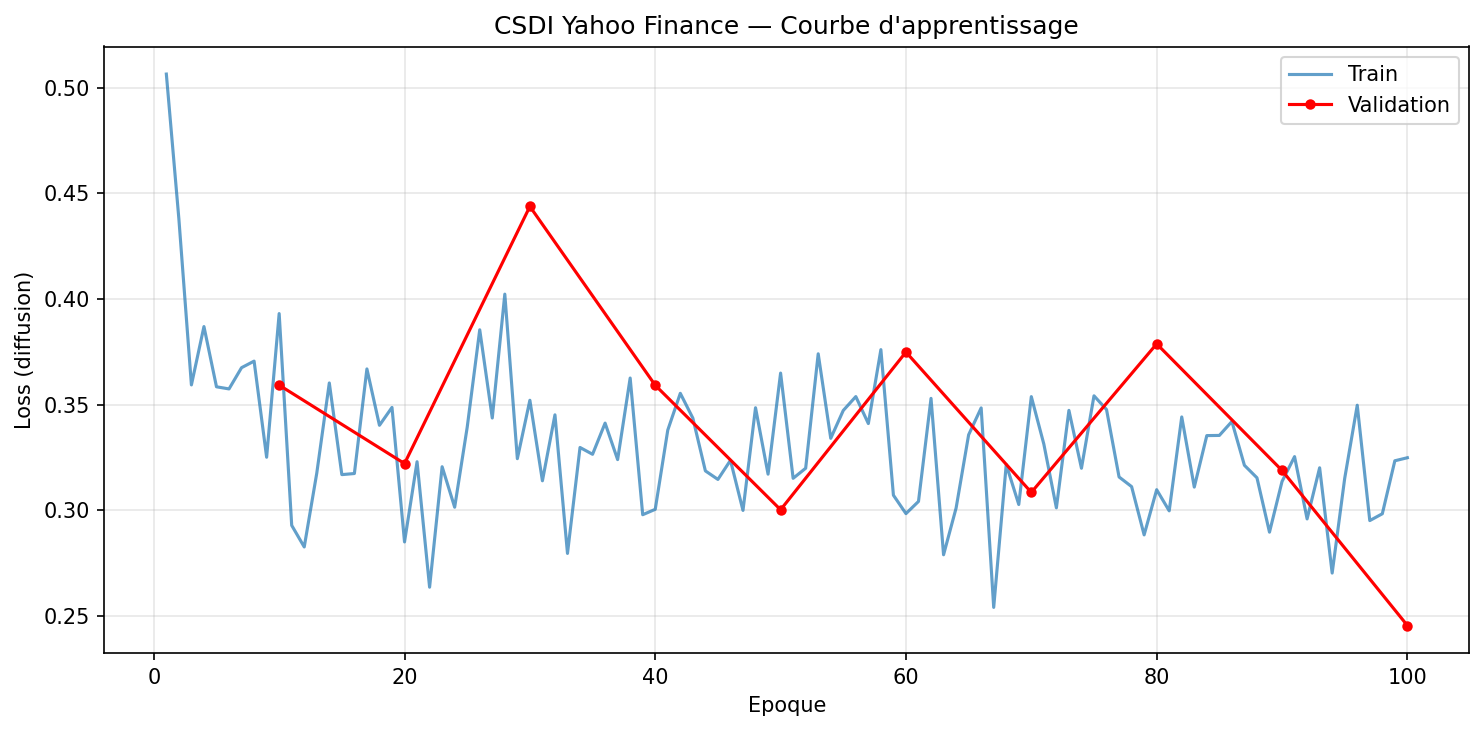
\includegraphics[width=0.85\linewidth]{23_csdi_yahoo_training_loss.png}
\caption{Courbe d'entra\^inement CSDI --- Yahoo Finance (100 \'epoques)}
\label{fig:csdi_loss_yahoo}
\end{figure}

\begin{figure}[H]
\centering
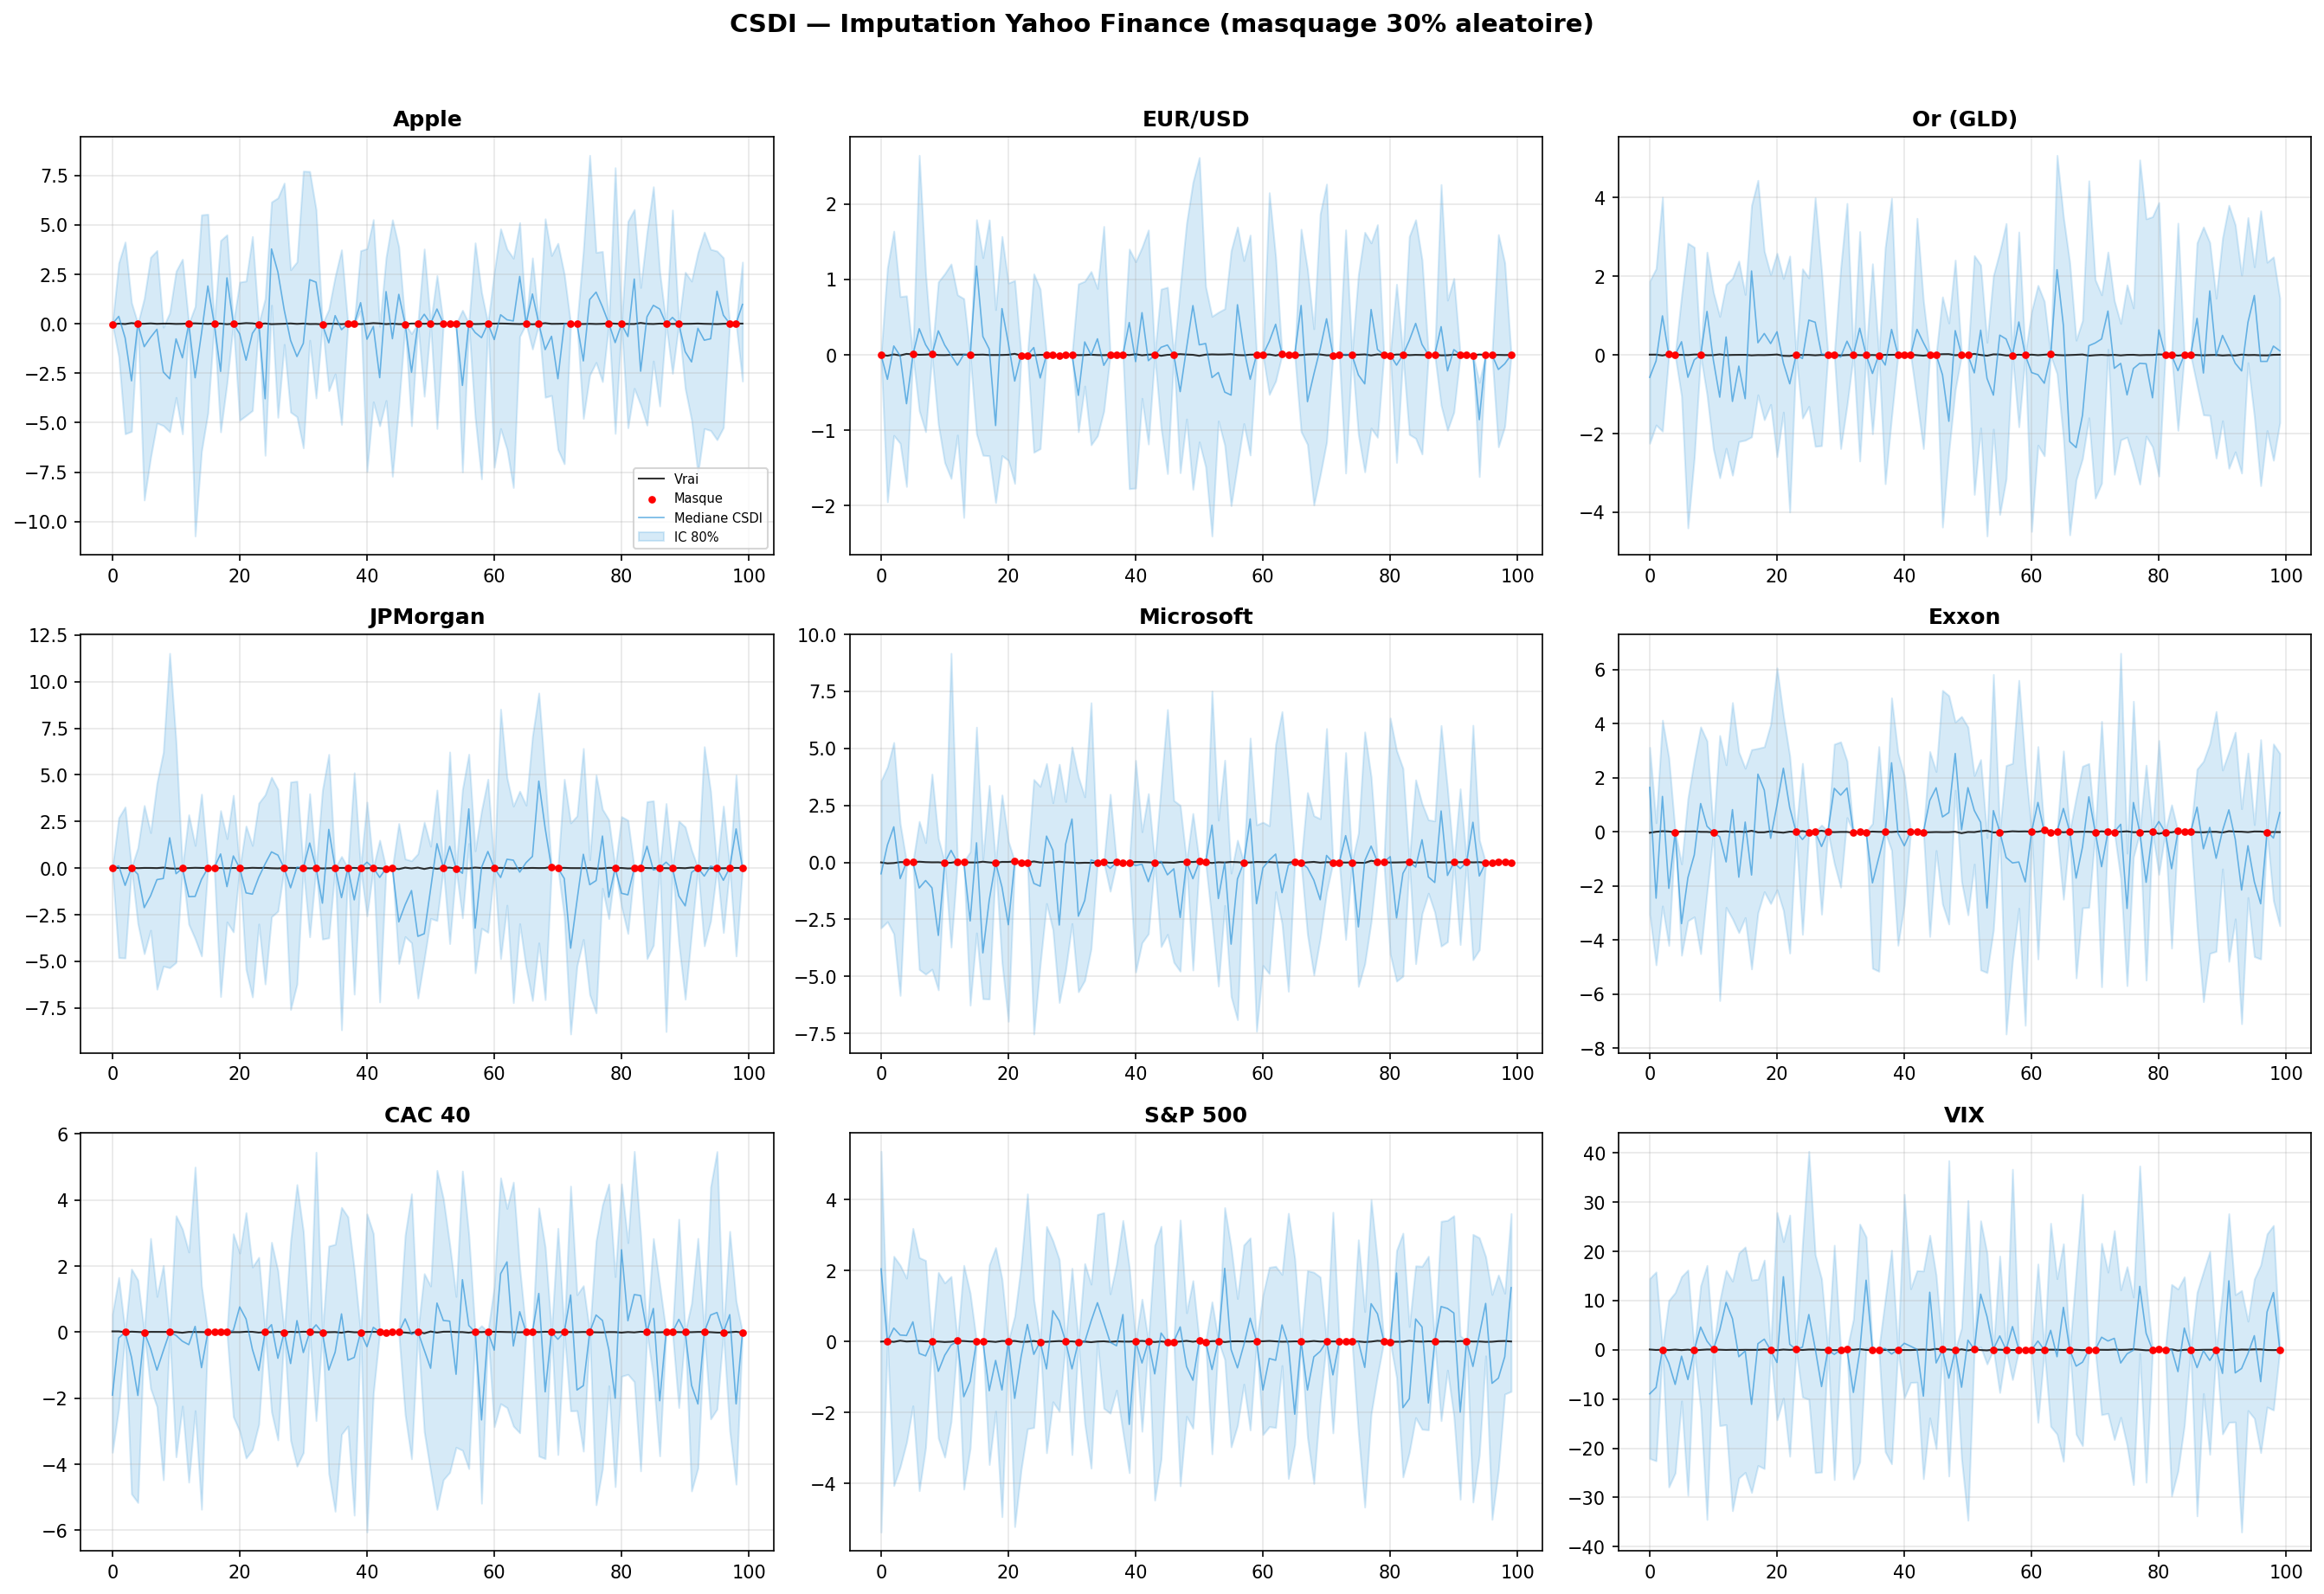
\includegraphics[width=0.95\linewidth]{24_csdi_yahoo_imputation.png}
\caption{Imputation CSDI --- Yahoo Finance : exemple avec IC \`a 80\%}
\label{fig:csdi_imputation_yahoo}
\end{figure}

\begin{figure}[H]
\centering
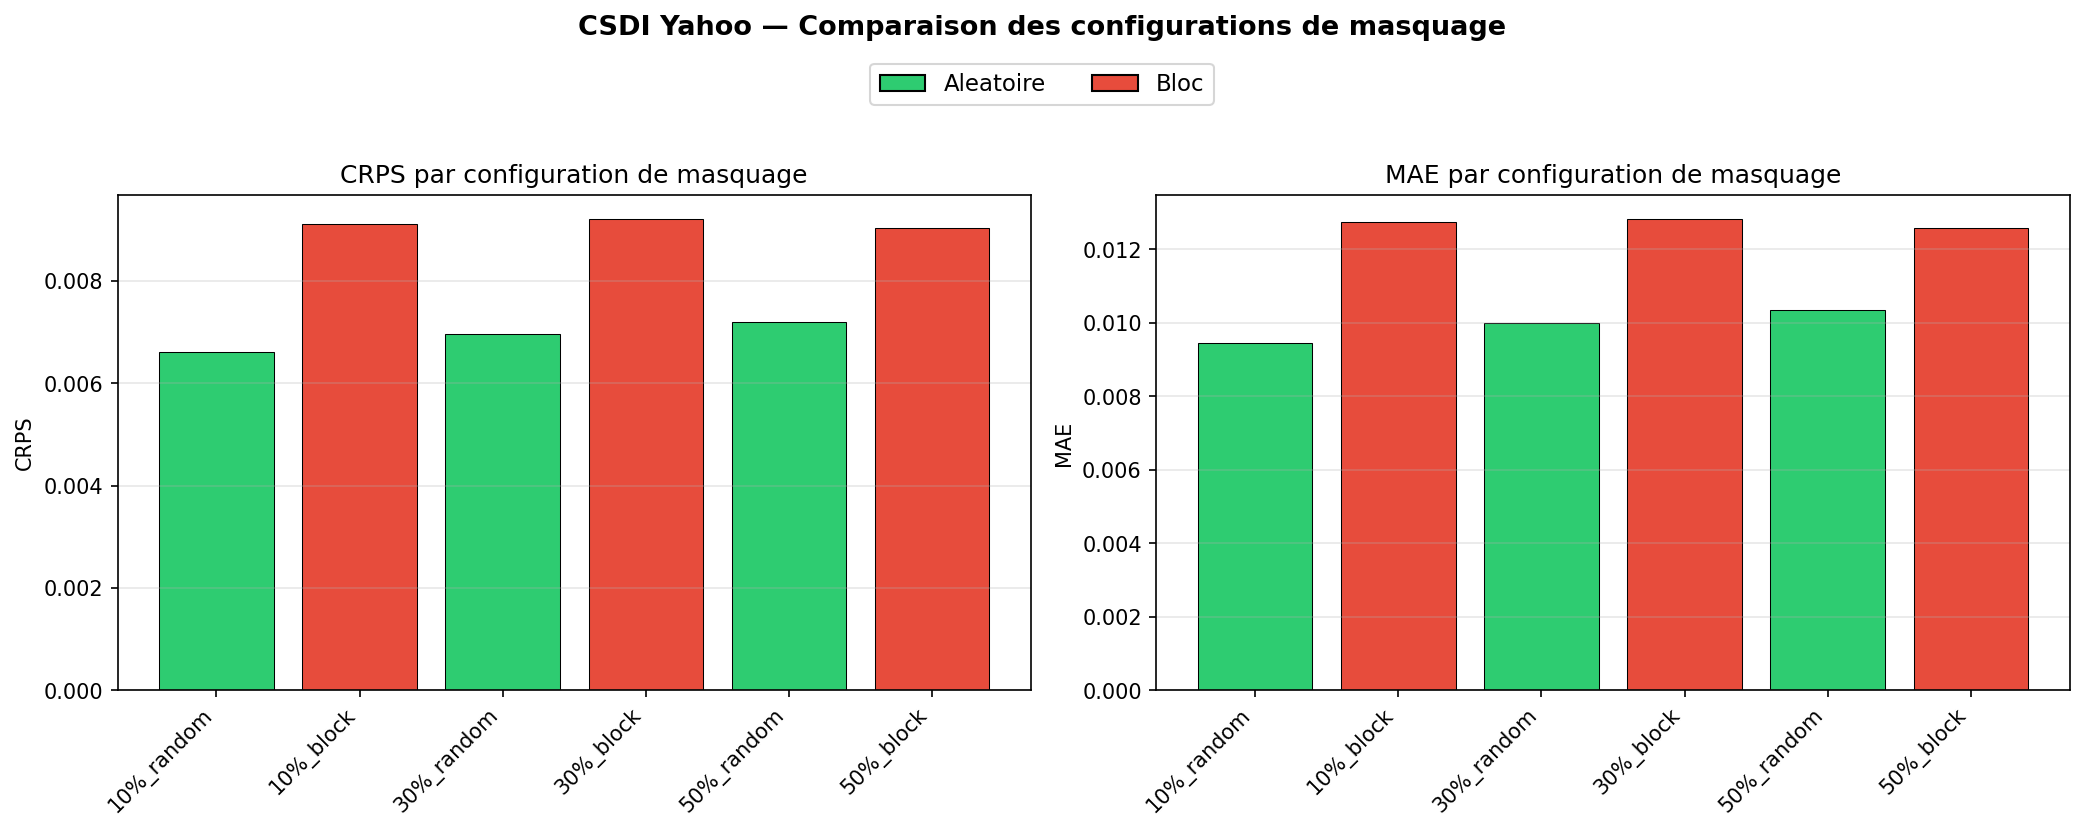
\includegraphics[width=0.95\linewidth]{25_csdi_yahoo_masking_comparison.png}
\caption{Comparaison des configurations de masquage --- Yahoo Finance}
\label{fig:csdi_masking_yahoo}
\end{figure}

\subsection{Interpr\'etabilit\'e SHAP}

L'analyse SHAP sur XGBoost et LightGBM pour la pr\'ediction du S\&P 500 \`a $h{+}1$ r\'ev\`ele :

\begin{itemize}
    \item \textbf{Feature individuelle la plus influente} : la Figure~\ref{fig:shap_summary} montre que \texttt{JPMorgan\_t-14} arrive en t\^ete pour XGBoost, suivie de \texttt{VIX\_t-17} et \texttt{Apple\_t-1}. Les features les plus importantes ne sont donc \textbf{pas toutes des lags r\'ecents} --- des lags \'eloign\'es ($t{-}14$, $t{-}17$) apparaissent en t\^ete, sugg\'erant que XGBoost capture des motifs \`a plus long terme
    \item \textbf{Par s\'erie agr\'eg\'ee} (Figure~\ref{fig:shap_xgb_lgb}) : pour XGBoost, Exxon domine, suivie d'Apple et JPMorgan. Pour LightGBM, Exxon domine \'egalement, mais le S\&P 500 passe au 2\textsuperscript{e} rang (8\textsuperscript{e} chez XGBoost) et CAC 40 au 3\textsuperscript{e} (5\textsuperscript{e} chez XGBoost). Les \textbf{classements diff\`erent significativement} au-del\`a du 1\textsuperscript{er} rang, refl\'etant les strat\'egies de split diff\'erentes des deux algorithmes
    \item \textbf{Importance par lag} (Figure~\ref{fig:shap_decomp}b) : la d\'ecroissance n'est \textbf{pas monotone} --- l'importance est irr\'eguli\`ere avec un pic marqu\'e \`a $t{-}7$ et des remontees aux lags \'eloign\'es ($t{-}15$ \`a $t{-}20$). Ce profil ne correspond pas \`a une d\'ecroissance exponentielle simple
\end{itemize}

\begin{figure}[H]
\centering
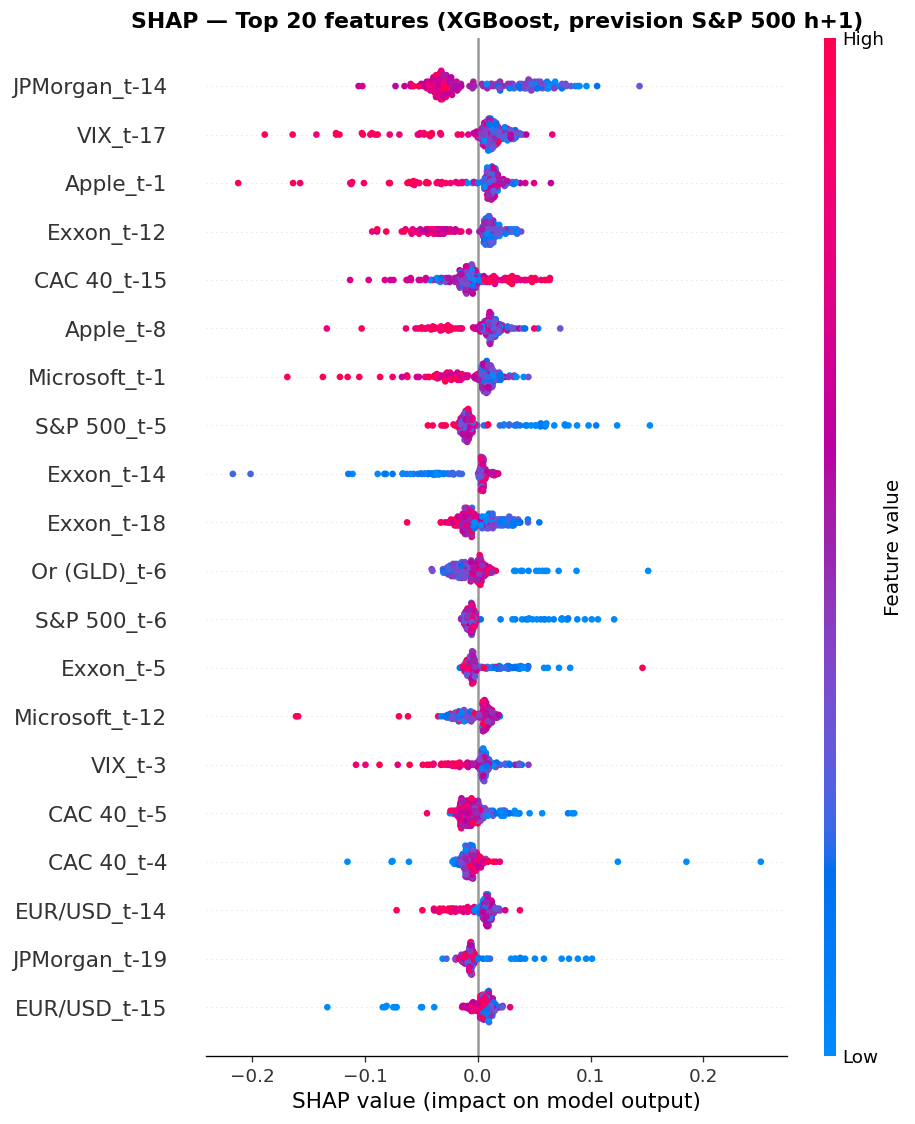
\includegraphics[width=0.95\linewidth]{18_shap_summary_xgboost.png}
\caption{SHAP Summary Plot --- XGBoost (pr\'ediction S\&P 500 \`a h+1)}
\label{fig:shap_summary}
\end{figure}

\begin{figure}[H]
\centering
\begin{subfigure}[b]{0.48\linewidth}
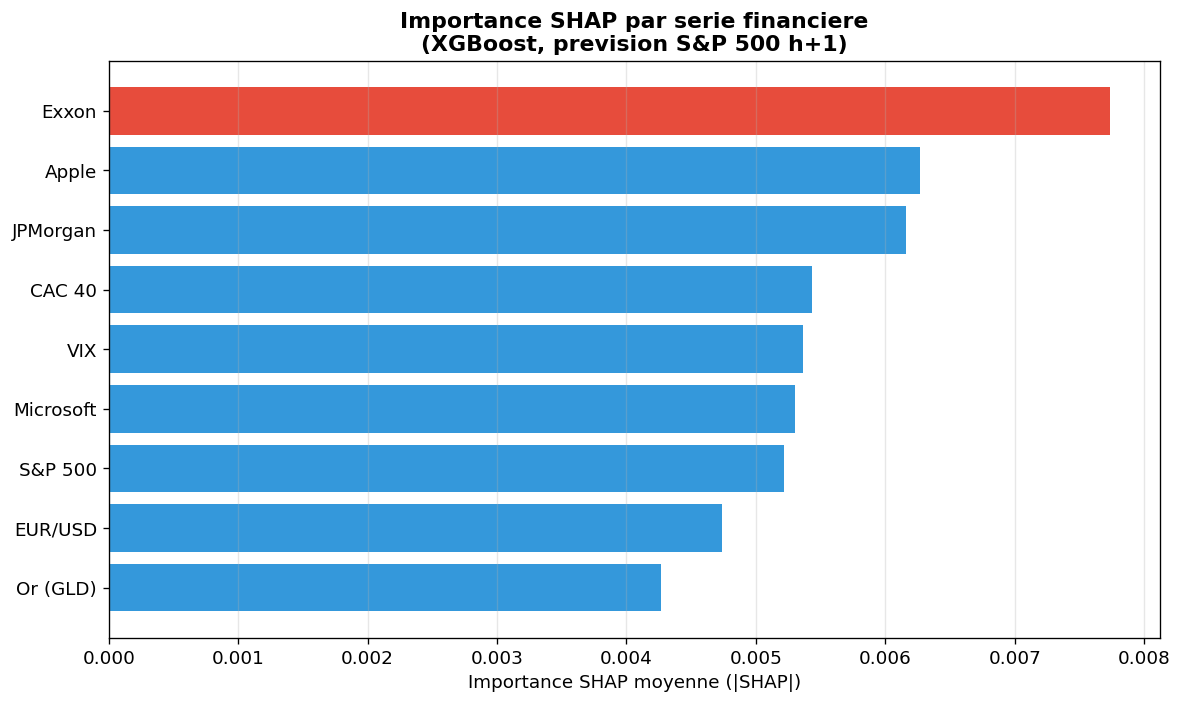
\includegraphics[width=\linewidth]{19_shap_importance_par_serie.png}
\caption{Importance par s\'erie}
\end{subfigure}
\hfill
\begin{subfigure}[b]{0.48\linewidth}
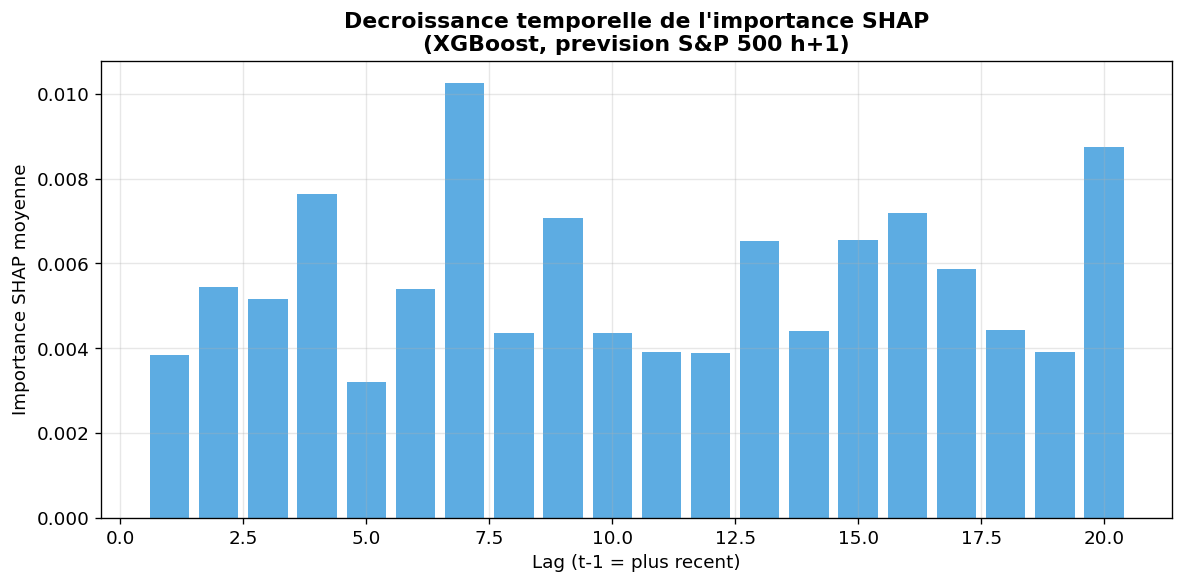
\includegraphics[width=\linewidth]{20_shap_importance_par_lag.png}
\caption{Importance par lag}
\end{subfigure}
\caption{D\'ecomposition SHAP : importance agr\'eg\'ee par s\'erie et par lag}
\label{fig:shap_decomp}
\end{figure}

\begin{figure}[H]
\centering
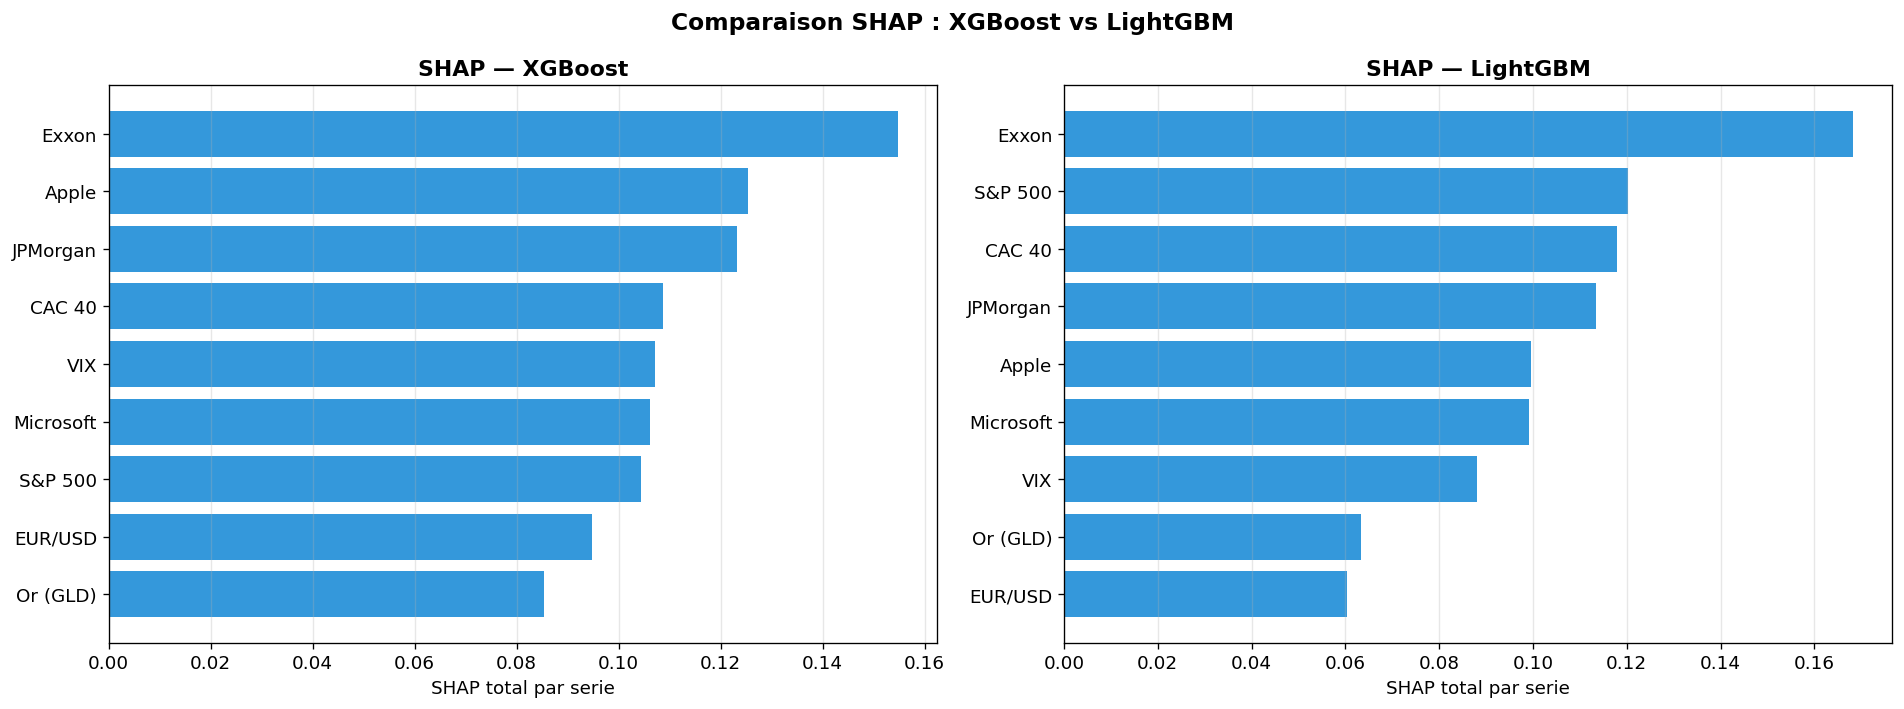
\includegraphics[width=0.85\linewidth]{22_shap_xgb_vs_lgb.png}
\caption{Comparaison SHAP : XGBoost vs.\ LightGBM}
\label{fig:shap_xgb_lgb}
\end{figure}

\subsection{Test de Diebold-Mariano}

Le test de Diebold-Mariano est appliqu\'e \`a toutes les paires de 6 mod\`eles (Zero, Na\"if, ARIMA refitt\'e par fen\^etre, XGBoost, LightGBM, LSTM). La variance de la statistique DM est estim\'ee avec un \textbf{estimateur HAC de Newey-West} \cite{newey1987} (noyau de Bartlett, troncature \`a $H{-}1 = 4$ retards) pour corriger l'autocorr\'elation induite par le chevauchement des fen\^etres glissantes. La heatmap ci-dessous montre les statistiques DM et les p-valeurs associ\'ees.

\begin{figure}[H]
\centering
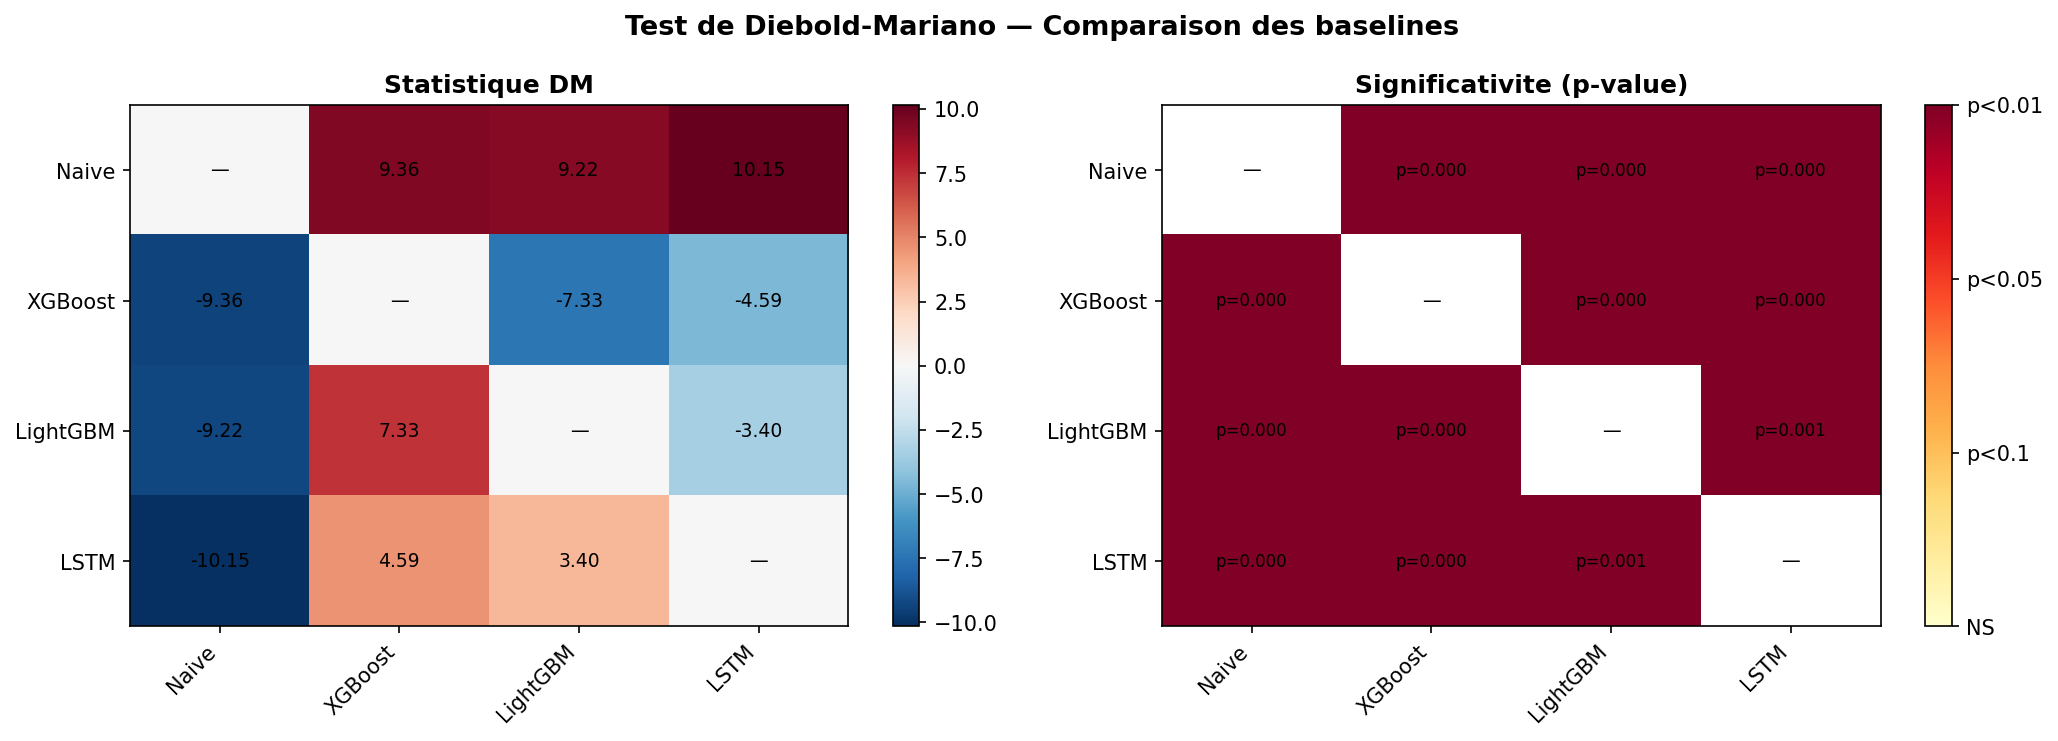
\includegraphics[width=0.85\linewidth]{26_diebold_mariano.png}
\caption{Heatmap du test de Diebold-Mariano --- statistiques DM pour toutes les paires}
\label{fig:dm_test}
\end{figure}

\textbf{Interpr\'etation :} Le test DM avec correction HAC (Newey-West) r\'ev\`ele que :
\begin{itemize}
    \item Le baseline z\'ero et XGBoost ne sont \textbf{pas significativement diff\'erents} (DM $= -0.22$, $p > 0.1$), confirmant que sur des log-rendements normalis\'es centr\'es, pr\'edire z\'ero est une strat\'egie comp\'etitive.
    \item LightGBM est significativement \textbf{moins bon} que le z\'ero (DM $= -5.03$, $p < 0.01$), sugg\'erant un l\'eger sur-apprentissage.
    \item ARIMA (refitt\'e par fen\^etre) est significativement inf\'erieur au z\'ero (DM $= -5.18$, $p < 0.01$).
    \item Le baseline na\"if (derni\`ere valeur) est significativement pire que tous les autres mod\`eles ($|$DM$| > 10$, $p < 0.01$).
    \item LightGBM surpasse significativement ARIMA (DM $= -3.76$, $p < 0.01$) mais est significativement inf\'erieur \`a XGBoost (DM $= 5.90$, $p < 0.01$).
\end{itemize}

% ══════════════════════════════════════════════════════════
% 5. DISCUSSION
% ══════════════════════════════════════════════════════════
\section{Discussion}

\subsection{Avantages de l'approche CSDI}

\begin{enumerate}
    \item \textbf{Flexibilit\'e} : CSDI peut th\'eoriquement g\'erer imputation et pr\'evision dans un cadre unifi\'e (la pr\'evision \'etant formul\'ee comme une imputation des positions futures). \textbf{Limite :} dans ce projet, nous n'avons \'evalu\'e CSDI que sur la t\^ache d'imputation ; la pr\'evision probabiliste par diffusion n'a pas \'et\'e impl\'ement\'ee, et les baselines de pr\'evision (Table~3) ne sont donc pas directement comparables \`a CSDI
    \item \textbf{Quantification native de l'incertitude} : les intervalles de confiance d\'ecoulent directement de l'\'echantillonnage, sans hypoth\`ese param\'etrique suppl\'ementaire
    \item \textbf{Capture des d\'ependances multivari\'ees} : l'architecture \`a attention mod\'elise les corr\'elations entre s\'eries
    \item \textbf{Comportement selon le masquage} : en mode al\'eatoire, la performance se d\'egrade l\'eg\`erement avec le taux de masquage (RMSE Yahoo : 0.0198 \`a 10\% $\to$ 0.0220 \`a 50\%). En mode bloc, le RMSE reste stable (0.0276 $\to$ 0.0284), sugg\'erant que le mod\`ele exploite peu la longueur du contexte restant
\end{enumerate}

\subsection{Limites}

\begin{enumerate}
    \item \textbf{Co\^ut computationnel} : 50 pas de diffusion $\times$ 50 \'echantillons rendent l'inf\'erence lente ($\sim$10 secondes par fen\^etre sur GPU) compar\'ee aux baselines ($<$ 1 ms)
    \item \textbf{Entra\^inement} : 100 \'epoques ($\sim$30 minutes sur GPU RTX 4050), contre quelques secondes pour XGBoost/LightGBM
    \item \textbf{Interpr\'etabilit\'e} : le processus de diffusion est opaque --- SHAP ne peut pas \^etre appliqu\'e directement au d\'ebruitage it\'eratif, contrairement aux mod\`eles \`a base d'arbres
    \item \textbf{Pr\'evision non r\'ealis\'ee} : l'objectif de pr\'evision probabiliste par diffusion (formuler la pr\'evision comme imputation des positions futures) n'a pas \'et\'e impl\'ement\'e dans ce projet. Seule l'imputation est \'evalu\'ee pour CSDI
    \item \textbf{Sous-dispersion des IC} : la couverture empirique des IC \`a 80\% n'atteint que 50--61\% selon la configuration (Table~\ref{tab:coverage}), indiquant que les intervalles pr\'edits sont trop \'etroits. Avec seulement 10 \'echantillons, les quantiles $q_{10}$ et $q_{90}$ sont estim\'es de mani\`ere bruit\'ee
    \item \textbf{Hypoth\`eses sur les manquants} : notre \'evaluation simule des manquants MCAR (al\'eatoire) et MCAR structur\'e (bloc contigu mais ind\'ependant des valeurs), mais ne teste pas les m\'ecanismes MAR ou MNAR, plus r\'ealistes pour les donn\'ees financi\`eres
    \item \textbf{Queues \'epaisses non mod\'elis\'ees} : CSDI suppose implicitement un bruit gaussien lors de la diffusion. Les queues \'epaisses des rendements financiers pourraient n\'ecessiter des distributions alternatives (Student-$t$)
\end{enumerate}

\subsection{Comparaison des approches probabilistes}

\begin{table}[H]
\centering
\caption{Comparaison des m\'ethodes de quantification de l'incertitude}
\begin{tabular}{lll}
\toprule
\textbf{M\'ethode} & \textbf{Approche} & \textbf{Mod\`eles} \\
\midrule
\'Echantillonnage par diffusion & Natif & CSDI \\
R\'egression quantile & Post-hoc & XGBoost, LightGBM \\
\textit{(non disponible)} & --- & LSTM, ARIMA, Na\"if \\
\bottomrule
\end{tabular}
\end{table}

% ══════════════════════════════════════════════════════════
% 6. CONCLUSION
% ══════════════════════════════════════════════════════════
\section{Conclusion}

Ce projet a explor\'e l'application des mod\`eles de diffusion conditionnels (CSDI) \`a l'imputation de s\'eries temporelles financi\`eres. Les principaux apports sont :

\begin{itemize}
    \item Une impl\'ementation compl\`ete de CSDI sur deux jeux de donn\'ees financiers r\'eels
    \item Une comparaison des baselines de pr\'evision (6 mod\`eles incluant le z\'ero) et une comparaison statistique par test DM
    \item Des baselines d'imputation (z\'ero, interpolation lin\'eaire) permettant de contextualiser les r\'esultats CSDI
    \item Une analyse d'interpr\'etabilit\'e SHAP sur les mod\`eles \`a base d'arbres
    \item Une application Streamlit interactive pour la d\'emonstration
\end{itemize}

Les r\'esultats montrent que CSDI excelle en masquage al\'eatoire : il bat le z\'ero et l'interpolation sur Yahoo Finance (RMSE 0.0205 vs z\'ero 0.0275) et toutes les baselines sur Exchange Rate (RMSE 0.0035 vs interpolation 0.0040). Cependant, la gaussienne conditionnelle --- une baseline sans apprentissage --- bat CSDI sur Yahoo en masquage al\'eatoire (RMSE 0.0188 vs 0.0198) en exploitant les corr\'elations inter-s\'eries. En masquage bloc, le z\'ero reprend l'avantage sur Yahoo (RMSE 0.0265--0.0276 vs CSDI 0.0276--0.0284) et l'interpolation sur Exchange Rate (0.0108 vs 0.0126), montrant que CSDI excelle sur les masquages dispers\'es mais p\^atit des longues lacunes.

\textbf{Limites principales :} l'objectif de pr\'evision probabiliste par diffusion n'a pas \'et\'e r\'ealis\'e (seule l'imputation est \'evalu\'ee pour CSDI), les IC \`a 80\% sont sous-dispersifs (couverture empirique de 50--61\% au lieu de 80\%), et les queues \'epaisses des distributions financi\`eres ne sont pas mod\'elis\'ees explicitement.

\textbf{Perspectives :} impl\'ementer la pr\'evision par diffusion (en masquant les positions futures), am\'eliorer la couverture des IC (augmenter le nombre d'\'echantillons, recalibration post-hoc), explorer des processus de diffusion \`a queues \'epaisses, et \'etendre l'\'evaluation \`a des m\'ecanismes de donn\'ees manquantes MAR.

% ══════════════════════════════════════════════════════════
% REFERENCES
% ══════════════════════════════════════════════════════════
\newpage
\begin{thebibliography}{99}

\bibitem{tashiro2021}
Y.~Tashiro, J.~Song, Y.~Song, and S.~Ermon,
``CSDI: Conditional Score-based Diffusion Models for Probabilistic Time Series Imputation,''
\textit{Advances in Neural Information Processing Systems (NeurIPS)}, 2021.

\bibitem{ho2020}
J.~Ho, A.~Jain, and P.~Abbeel,
``Denoising Diffusion Probabilistic Models,''
\textit{Advances in Neural Information Processing Systems (NeurIPS)}, 2020.

\bibitem{sohl2015}
J.~Sohl-Dickstein, E.~Weiss, N.~Maheswaranathan, and S.~Ganguli,
``Deep Unsupervised Learning using Nonequilibrium Thermodynamics,''
\textit{International Conference on Machine Learning (ICML)}, 2015.

\bibitem{vaswani2017}
A.~Vaswani, N.~Shazeer, N.~Parmar, J.~Uszkoreit, L.~Jones, A.N.~Gomez, L.~Kaiser, and I.~Polosukhin,
``Attention Is All You Need,''
\textit{Advances in Neural Information Processing Systems (NeurIPS)}, 2017.

\bibitem{chen2016}
T.~Chen and C.~Guestrin,
``XGBoost: A Scalable Tree Boosting System,''
\textit{ACM SIGKDD International Conference on Knowledge Discovery and Data Mining}, 2016.

\bibitem{ke2017}
G.~Ke, Q.~Meng, T.~Finley, T.~Wang, W.~Chen, W.~Ma, Q.~Ye, and T.-Y.~Liu,
``LightGBM: A Highly Efficient Gradient Boosting Decision Tree,''
\textit{Advances in Neural Information Processing Systems (NeurIPS)}, 2017.

\bibitem{hochreiter1997}
S.~Hochreiter and J.~Schmidhuber,
``Long Short-Term Memory,''
\textit{Neural Computation}, 9(8):1735--1780, 1997.

\bibitem{lundberg2017}
S.M.~Lundberg and S.-I.~Lee,
``A Unified Approach to Interpreting Model Predictions,''
\textit{Advances in Neural Information Processing Systems (NeurIPS)}, 2017.

\bibitem{lundberg2020}
S.M.~Lundberg, G.~Erion, H.~Chen, A.~DeGrave, J.M.~Prutkin, B.~Nair, R.~Katz, J.~Himmelfarb, N.~Bansal, and S.-I.~Lee,
``From Local Explanations to Global Understanding with Explainable AI for Trees,''
\textit{Nature Machine Intelligence}, 2(1):56--67, 2020.

\bibitem{diebold1995}
F.X.~Diebold and R.S.~Mariano,
``Comparing Predictive Accuracy,''
\textit{Journal of Business \& Economic Statistics}, 13(3):253--263, 1995.

\bibitem{harvey1997}
D.~Harvey, S.~Leybourne, and P.~Newbold,
``Testing the Equality of Prediction Mean Squared Errors,''
\textit{International Journal of Forecasting}, 13(2):281--291, 1997.

\bibitem{newey1987}
W.K.~Newey and K.D.~West,
``A Simple, Positive Semi-Definite, Heteroskedasticity and Autocorrelation Consistent Covariance Matrix,''
\textit{Econometrica}, 55(3):703--708, 1987.

\bibitem{cont2001}
R.~Cont,
``Empirical Properties of Asset Returns: Stylized Facts and Statistical Issues,''
\textit{Quantitative Finance}, 1(2):223--236, 2001.

\bibitem{rubin1976}
D.B.~Rubin,
``Inference and Missing Data,''
\textit{Biometrika}, 63(3):581--592, 1976.

\bibitem{box1970}
G.E.P.~Box and G.M.~Jenkins,
\textit{Time Series Analysis: Forecasting and Control},
Holden-Day, 1970.

\bibitem{salinas2020}
D.~Salinas, V.~Flunkert, J.~Gasthaus, and T.~Januschowski,
``DeepAR: Probabilistic Forecasting with Autoregressive Recurrent Networks,''
\textit{International Journal of Forecasting}, 36(3):1181--1191, 2020.

\bibitem{rasul2021}
K.~Rasul, A.-S.~Sheikh, I.~Schuster, U.~Bergmann, and R.~Vollgraf,
``Multivariate Probabilistic Time Series Forecasting via Conditioned Normalizing Flows,''
\textit{International Conference on Learning Representations (ICLR)}, 2021.

\bibitem{rasul2021tg}
K.~Rasul, C.~Seward, I.~Schuster, and R.~Vollgraf,
``Autoregressive Denoising Diffusion Models for Multivariate Probabilistic Time Series Forecasting,''
\textit{International Conference on Machine Learning (ICML)}, 2021.

\bibitem{zhou2021}
H.~Zhou, S.~Zhang, J.~Peng, S.~Zhang, J.~Li, H.~Xiong, and W.~Zhang,
``Informer: Beyond Efficient Transformer for Long Sequence Time-Series Forecasting,''
\textit{AAAI Conference on Artificial Intelligence}, 2021.

\bibitem{oord2016}
A.~van~den~Oord, S.~Dieleman, H.~Zen, K.~Simonyan, O.~Vinyals, A.~Graves, N.~Kalchbrenner, A.~Senior, and K.~Kavukcuoglu,
``WaveNet: A Generative Model for Raw Audio,''
\textit{arXiv preprint arXiv:1609.03499}, 2016.

\bibitem{yahoo2026}
Yahoo Finance,
``Historical Market Data,''
\url{https://finance.yahoo.com/}, acc\`es 2026.

\bibitem{lai2018}
G.~Lai, W.-C.~Chang, Y.~Yang, and H.~Liu,
``Modeling Long- and Short-Term Temporal Patterns with Deep Neural Networks,''
\textit{International ACM SIGIR Conference}, 2018.
\textit{(Source du jeu de donn\'ees Exchange Rate)}

\end{thebibliography}

\end{document}
